
\documentclass[a4paper,11pt]{article}%,twocolumn
%% packages

\usepackage{blindtext} % needed for creating dummy text passages
%\usepackage{ngerman} % needed for German default language
\usepackage{amsmath} % needed for command eqref
\usepackage{amssymb} % needed for math fonts
\usepackage[colorlinks=true,breaklinks]{hyperref} % needed for creating hyperlinks in the document, the option colorlinks=true gets rid of the awful boxes, breaklinks breaks lonkg links (list of figures), and ngerman sets everything for german as default hyperlinks language
\usepackage[hyphenbreaks]{breakurl} % ben�tigt f�r das Brechen von URLs in Literaturreferenzen, hyphenbreaks auch bei links, die �ber eine Seite gehen (mit hyphenation).
\usepackage{xcolor}
\definecolor{c1}{rgb}{0,0,1} % blue
\definecolor{c2}{rgb}{0,0.3,0.9} % light blue
\definecolor{c3}{rgb}{0.3,0,0.9} % red blue
\hypersetup{
    linkcolor={c1}, % internal links
    citecolor={c2}, % citations
    urlcolor={c3} % external links/urls
}
%\usepackage{cite} % needed for cite
\usepackage[square,authoryear]{natbib} % needed for cite and abbrvnat bibliography style
\usepackage[nottoc]{tocbibind} % needed for displaying bibliography and other in the table of contents
\usepackage{graphicx} % needed for \includegraphics 
\usepackage{longtable} % needed for long tables over pages
\usepackage{bigstrut} % needed for the command \bigstrut
\usepackage{enumerate} % needed for some options in enumerate
%\usepackage{todonotes} % needed for todos
\usepackage{makeidx} % needed for creating an index
\makeindex
\usepackage{gensymb}
\usepackage{url}
\usepackage{psfrag}
\usepackage{multirow}
\usepackage{subfigure}
%% page settings

\usepackage[top=20mm, bottom=20mm,left=15mm,right=15mm]{geometry} % needed for page border settings
\parindent=0mm % for space of first line of new text block
\sloppy % for writing with hyphenless justification (tries to)
\hyphenation{} % use hyphenation of tolerance parametershttp://www.jr-x.de/publikationen/latex/tipps/zeilenumbruch.html
\hyphenpenalty=10000
\exhyphenpenalty=10000
\usepackage{fancyhdr} % needed for head and foot options
%% my macros

%% Text fomats
\newcommand{\tbi}[1]{\textbf{\textit{#1}}}

%% Math fonts
\newcommand{\bbA}{\mathbb{A}}
\newcommand{\bbB}{\mathbb{B}}
\newcommand{\bbC}{\mathbb{C}}
\newcommand{\bbD}{\mathbb{D}}
\newcommand{\bbE}{\mathbb{E}}
\newcommand{\bbF}{\mathbb{F}}
\newcommand{\bbG}{\mathbb{G}}
\newcommand{\bbH}{\mathbb{H}}
\newcommand{\bbI}{\mathbb{I}}
\newcommand{\bbJ}{\mathbb{J}}
\newcommand{\bbK}{\mathbb{K}}
\newcommand{\bbL}{\mathbb{L}}
\newcommand{\bbM}{\mathbb{M}}
\newcommand{\bbN}{\mathbb{N}}
\newcommand{\bbO}{\mathbb{O}}
\newcommand{\bbP}{\mathbb{P}}
\newcommand{\bbQ}{\mathbb{Q}}
\newcommand{\bbR}{\mathbb{R}}
\newcommand{\bbS}{\mathbb{S}}
\newcommand{\bbT}{\mathbb{T}}
\newcommand{\bbU}{\mathbb{U}}
\newcommand{\bbV}{\mathbb{V}}
\newcommand{\bbW}{\mathbb{W}}
\newcommand{\bbX}{\mathbb{X}}
\newcommand{\bbY}{\mathbb{Y}}
\newcommand{\bbZ}{\mathbb{Z}}
\usepackage[ framed, numbered]{matlab-prettifier}%framed,%
\usepackage{listings}
\usepackage{physics}
\usepackage{pdfpages}
\usepackage[toc,page]{appendix}
\usepackage{float}
\usepackage{hyperref}

% for code
\usepackage{listings}
\usepackage{color}
% Define colors
\definecolor{codegreen}{rgb}{0,0.6,0}
\definecolor{codegray}{rgb}{0.5,0.5,0.5}
\definecolor{codepurple}{rgb}{0.58,0,0.82}
\definecolor{backcolour}{rgb}{0.95,0.95,0.92}
% Setup the listings package
\lstset{
    backgroundcolor=\color{backcolour},   
    commentstyle=\color{codegreen},
    keywordstyle=\color{magenta},
    numberstyle=\tiny\color{codegray},
    stringstyle=\color{codepurple},
    basicstyle=\footnotesize,
    breakatwhitespace=false,         
    breaklines=true,                 
    captionpos=b,                    
    keepspaces=true,                 
    numbers=left,                    
    numbersep=5pt,                  
    showspaces=false,                
    showstringspaces=false,
    showtabs=false,                  
    tabsize=2
}

\newenvironment{qanda}{\setlength{\parindent}{0pt}}{\bigskip}
\newcommand{\Q}{\bigskip\bfseries Q: }
\newcommand{\A}{\par\textbf{Answer: } \normalfont}

\begin{document}
\begin{titlepage}
\center % Center everything on the page

%-------------------------------------------------------------------------------------
%	HEADING SECTIONS
%------------------------------------------------------------------------------------
\textbf{\large Department of Electrical and Computer Engineering}\\[0.5cm]
\textbf{\Large University of Colorado at Boulder}\\[1cm]
\textbf{\large ECEN5623 - Real Time Embedded Systems }\\[2cm]

\includegraphics[width=0.3\textwidth]{figures/cu}\\[2cm]

	
%-------------------------------------------------------------------------------------
%	TITLE SECTION
%------------------------------------------------------------------------------------
\textbf{\Huge Exercise 5 }\\[0.2cm]



%----------------------------------------------------------------------------------------
%	MEMBERS SECTION
%----------------------------------------------------------------------------------------


\vfill

\textbf{\large Submitted by}\\[0.5cm]

{\large Parth | Jithedra}\\[0.5cm]	

%----------------------------------------------------------------------------------------
%	DATE SECTION
%----------------------------------------------------------------------------------------

\textbf{\large Submitted on}
\textbf{\Large \today} % Date, change the \today to a set date if you want to be precise

%----------------------------------------------------------------------------------------

\vfill % Fill the rest of the page with whitespace

\end{titlepage}


\pagebreak

\tableofcontents
\listoffigures
\listoftables
\vfill
\begin{center}
	\textbf{\textit{*PDF is clickable}}
\end{center}

\pagebreak

\section*{Objective}
\begin{enumerate}
	\item Understanding the concept of the Cyclic Executive in comparison to Linux POSIX RT threading and RTOS.
	      Implementing and analyzing custom feasibility test code for different scheduling policies (RM, EDF, LLF) using Cheddar.
	\item Moreover, understanding the constraints, assumptions, and derivation steps in Rate Monotonic (RM) Least Upper Bound (LUB) as outlined in Chapter 3 of the textbook.

\end{enumerate}

\pagebreak
\begin{qanda}
	\section{Question 1}
	\begin{enumerate}
		\item[] \Q [10 points] [All papers here also on Canvas] Read Sha, Rajkumar, et al paper, "Priority Inheritance Protocols: An Approach to Real-Time Synchronization"
			\begin{enumerate}
				\addcontentsline{toc}{subsection}{A}
				\item \Q Summarize 3 main key points the paper makes. Read Dr. Siewert’s summary paper on the topic as well which might be easier to understand.

				      \A
				      This paper studies priority inheritance protocols, such as the basic and priority ceiling protocols, to address uncontrolled priority inversion. This occurs when a high-priority task is delayed by a low-priority task accessing a shared resource. The priority ceiling protocol limits the maximum blocking time of a high-priority task to the duration of the low-priority task, reducing the chance of deadlocks. Following are the 3 main key points the paper makes:\\
				      \begin{enumerate}
					      \item[] \textbf{Priority Inheritance Protocols:} Real-time systems face challenges in scheduling tasks effectively, especially when tasks need to share resources. Traditional synchronization methods, such as semaphores, can lead to priority inversion issues, where lower priority tasks hold up higher priority ones. Priority inheritance protocols offer a solution to this problem by dynamically adjusting the priorities of tasks to ensure that higher priority tasks are not unnecessarily delayed by lower priority ones.
					      \item[] \textbf{Basic Priority Inheritance Protocol:} The basic priority inheritance protocol temporarily boosts the priority of a lower priority task to match that of a higher priority one while it accesses a shared resource. This prevents priority inversion and helps ensure that tasks meet their deadlines. However, the basic protocol still has limitations, such as the potential for deadlocks and chains of blocking events, which can impact system reliability and predictability.
					      \item[] \textbf{Priority Ceiling Protocol:} To address the limitations of the basic protocol, the priority ceiling protocol introduces the concept of priority ceilings for shared resources. Each resource is assigned a maximum priority level, and when a task accesses the resource, its priority is temporarily raised to the ceiling level. This prevents lower priority tasks from blocking higher priority ones while still allowing for efficient resource sharing. A set of n periodic tasks can be scheduled using the priority ceiling protocol, if task priorities adhere to Rate Monotonic (RM) theory and specific conditions are met. Although the priority ceiling protocol introduces its own challenges, such as ceiling blocking, it offers a more robust solution compared to the basic protocol.
				      \end{enumerate}

				      In summary, priority inheritance protocols play a crucial role in ensuring the effective scheduling of tasks in real-time systems. By addressing issues such as priority inversion, these protocols help improve system reliability and meet performance requirements. The priority ceiling protocol offers a promising solution by introducing priority ceilings for shared resources, although it requires careful consideration of its implications for system design and implementation.



				      \addcontentsline{toc}{subsection}{B}
				\item \Q Read the historical positions of Linus Torvalds as described by Jonathan Corbet and Ingo Molnar and Thomas Gleixner on this topic as well. Take a position on this topic yourself and write at least one well supported paragraph or more to defend your position based on what we have learned in class. Does the PI-futex (Futex, Futexes are Tricky) that is
				      described by Ingo Molnar provide safe and accurate protection from un-bounded priority inversion as described in the paper? If not, what is different about it?

				      \A Linus Torvalds, the creator of Linux, firmly opposes using priority inheritance protocols to solve priority inversion. He suggests avoiding these protocols by designing software without locks or using carefully crafted locks to prevent priority inversion. However, this approach may not be practical for complex real-world applications where shared resources and task prioritization are essential.\\\\
				      In contrast, Ingo Molnar, a member of the kernel development community, believes that priority inheritance protocols are necessary and proposes using priority inheritance futexes (PI-Futex) to address priority inversion effectively. PI-Futexes work by temporarily boosting the priority of lower-priority tasks to prevent them from delaying higher-priority tasks indefinitely. This solution operates mainly in user space, providing efficient and precise protection against priority inversion.\\\\
				      \textbf{Our stance aligns more closely with Ingo Molnar's perspective}, advocating for the adoption of priority inheritance protocols in situations where priority inversion poses a significant risk. While Torvalds' argument against priority inheritance may apply in some cases, it overlooks the complexities of real-time systems and the need for efficient synchronization mechanisms.\\\\
				      \textbf{PI-Futex}
				      The PI-Futex, created by Ingo Molnar, is an advanced tool for dealing with uncontrolled priority inversion in real-time systems. It mainly works in user space, handling locking tasks quickly and efficiently without relying too much on the kernel. If there's a conflict over a shared resource, the PI-Futex boosts the priority of lower-priority tasks temporarily so that higher-priority tasks can keep moving smoothly.\\\\
				      However, it's not a perfect solution for all cases of priority inversion, especially when the issue stems from deeper kernel-level locking mechanisms like mutexes or semaphores. In those situations, priority inversion can still happen even if we are using PI-Futexes.\\\\
				      Despite its flaws, the PI-Futex shows promise in preventing uncontrolled priority inversion, especially in systems where most locking happens in user space. However, how well it works depends on how it's implemented and the specific context of the application. Other factors, such as the nature of kernel-level locking mechanisms and the complexity of system interactions, can also affect how effective PI-Futexes are in tackling priority inversion.


				      \addcontentsline{toc}{subsection}{C}
				\item \Q Note that more recently Red Hat has added support for priority ceiling emulation and
				      priority inheritance and has a great overview on use of these POSIX real-time extension
				      features here – general real-time overview. The key systems calls are\\
				      pthread\_mutexattr\_setprotocol, pthread\_mutexattr\_getprotocol as well as
				      pthread\_mutex\_setpriorityceiling and pthread\_mutex\_getpriorityceiling. Why did some
				      of the Linux community resist addition of priority ceiling and/or priority inheritance until
				      more recently? (Linux has been distributed since the early 1990’s and the problem and solutions were known before this).
				      \A The hesitation within the Linux community to adopt priority ceiling and priority inheritance features until more recently can be explained by a few reasons. Generally, in the world of Linux development, there's a reluctance to add new features because they might make things more complicated, less stable, or slower. Adding priority ceiling and inheritance to the kernel's scheduler and locking mechanisms could make the system more complex and might affect how well it runs and how easy it is to keep it running smoothly. There were also discussions about whether these features were really needed for most Linux uses, since Linux is used for many different things, not just real-time tasks.\\\\
				      Another reason for the hesitation is the belief that there are other ways to fix priority inversion issues without needing priority inheritance. Linus Torvalds, who created Linux, wasn't convinced that priority inheritance was necessary and thought there might be better solutions.\\\\
				      Additionally, there were concerns about how hard it would be to add these features to the Linux kernel and what problems it might cause. Making the kernel more complicated could lead to more bugs or security issues, which nobody wants.
				      Plus, there were other things that people wanted to work on in the Linux community, so priority ceiling and inheritance might not have been seen as a top priority.\\\\
				      But as people started to realize how important real-time capabilities were becoming for Linux, especially in areas like embedded systems and industrial automation, there was more demand for these features. Red Hat, a big player in the Linux world, recently added support for priority ceiling and inheritance, showing that the community is starting to take these needs seriously. As Linux keeps evolving, adding these features shows that people are recognizing the importance of making Linux work well for real-time tasks.


				      \addcontentsline{toc}{subsection}{D}
				\item \Q Given that there are two solutions to unbounded priority inversion, priority ceiling
				      emulation and priority inheritance, based upon your reading on support for both by
				      POSIX real-time extensions, which do you think is best to use and why?
				      \A
				      When deciding between priority ceiling emulation and priority inheritance to tackle unbounded priority inversion, it's essential to consider how each method works and their respective advantages and drawbacks. Priority inheritance temporarily boosts the priority of a task holding a resource, reducing the time higher-priority tasks are blocked. In contrast, priority ceiling emulation ensures that a task can only access a resource if its priority is equal to or higher than the highest-priority task that might use the resource, preventing priority inversion from happening.\\\\
				      The choice between the two methods depends on the specific needs and limitations of the system. Priority inheritance may seem simpler to implement and understand, but it could lead to unexpected scheduling outcomes if priorities are frequently elevated. Priority ceiling emulation, while more effective at preventing priority inversion, requires a deep understanding of the system's resource usage patterns to set appropriate ceiling priorities, which can be complex and prone to errors.
				      In systems with well-defined and unchanging resource access patterns, priority ceiling emulation might be preferable because it proactively prevents priority inversion. However, in dynamic systems or environments where predicting task-resource interactions is challenging, priority inheritance could offer more flexibility. Ultimately, the best choice depends on factors like system performance, complexity, and ease of maintenance in specific application and environment.


			\end{enumerate}

	\end{enumerate}




	\section{Question 2}
	\begin{enumerate}
		\item[] \Q [25 points] Review the terminology guide (glossary in the textbook)
			\begin{enumerate}
				\addcontentsline{toc}{subsection}{A}
				\item \Q Describe clearly what it means to write "thread safe" functions that are "re-entrant".
				      There are generally three main ways to do this:\\
				      \begin{enumerate}
					      \item pure functions that use only stack and have no global memory,
					      \item functions which use thread indexed global data,
					      \item functions which use shared memory global data, but synchronize access to it using a
					            MUTEX semaphore critical section wrapper
				      \end{enumerate}
				      \A

				      thread-safe functions that are re-entrant involves creating functions that can be safely called and executed by multiple threads simultaneously without causing data corruption or unpredictable behavior. A function is considered thread-safe if it can be safely invoked by multiple threads at the same time. A function is re-entrant if it can be interrupted in the middle of execution and safely called again \textbf{("re-entered")} before the previous executions are complete. For a function to be both thread-safe and re-entrant, we can use these three techniques
				      \begin{enumerate}
					      \item Pure Functions That Use Only Stack and Have No Global Memory
					            Pure functions depend solely on their input arguments and do not use or modify any shared state, including global variables or static data. Each thread's invocation of a pure function is completely independent of another's, as all necessary data is passed in as parameters, and any state is kept on the thread's own stack. Since there is no shared state and no side effects, pure functions are inherently thread-safe and re-entrant.

					      \item  Functions Which Use Thread-Indexed Global Data
					            These functions use global data that is indexed in such a way that each thread accesses a separate instance of the data. This can be achieved using thread-local storage (TLS), where each thread has its own instance of a variable. Although the data might be globally accessible within the process, each thread's view of the global data is unique and isolated, preventing data races and ensuring thread safety.


					      \item Functions Which Use Shared Memory Global Data, But Synchronize Access to It Using a MUTEX Semaphore Critical Section Wrapper
					            When functions need to access and modify shared global data, ensuring thread safety requires preventing multiple threads from modifying the data concurrently. This is typically achieved using mutual exclusion (mutex) locks or other synchronization primitives to create a critical section—a section of code that only one thread can execute at a time. Before a thread enters a critical section, it must acquire the mutex; when it's done, it releases the mutex. This ensures that only one thread at a time can access the shared data, preventing race conditions.

				      \end{enumerate}




				      \addcontentsline{toc}{subsection}{B}
				\item \Q Describe each method and how you would code it and how it would impact real-time
				      threads/tasks
				      \A

				      \begin{enumerate}
					      \item Pure Functions That Use Only Stack and Have No Global Memory
					            Pure functions depend solely on their input arguments and do not use or modify any shared state, including global variables or static data. Each thread's invocation of a pure function is completely independent of another's, as all necessary data is passed in as parameters, and any state is kept on the thread's own stack. Since there is no shared state and no side effects, pure functions are inherently thread-safe and re-entrant.
					            \begin{lstlisting}[language=C]
#include <stdio.h>
#include <pthread.h>

pthread_t threads[2];



void * task(void * arg){
  int counter = 0;
  for(int i=0; i<10000; i++){
	  counter++;
	  printf("Thread %ld, sharedCounter: %d\n", (long)arg, counter);
  }
  return NULL;

}



int main(){
  for (long i = 0; i < 2; i++) {
	  pthread_create(&threads[i], NULL, task, (void*)i);
  }

  for (int i = 0; i < 2; i++) {
	  pthread_join(threads[i], NULL);
  }
  return 0;
}
\end{lstlisting}
					      \item  Functions Which Use Thread-Indexed Global Data
					            These functions use global data that is indexed in such a way that each thread accesses a separate instance of the data. This can be achieved using thread-local storage (TLS), where each thread has its own instance of a variable. Although the data might be globally accessible within the process, each thread's view of the global data is unique and isolated, preventing data races and ensuring thread safety.

					            Example:
					            \begin{lstlisting}[language=C]
#include <stdio.h>
#include <pthread.h>

pthread_t threads[2];
// Thread-local indexed variable to store counter
__thread int counter = 0;


void* task(void * arg){
  for(int i=0; i<10000; i++){
	  counter++;
	  printf("Thread %ld, sharedCounter: %d\n", (long)arg, counter);
  }

  return NULL;

}



int main(){
  for (long i = 0; i < 2; i++) {
	  pthread_create(&threads[i], NULL, task, (void*)i);
  }

  for (int i = 0; i < 2; i++) {
	  pthread_join(threads[i], NULL);
  }
  return 0;
}
		\end{lstlisting}
					      \item Functions Which Use Shared Memory Global Data, But Synchronize Access to It Using a MUTEX Semaphore Critical Section Wrapper
					            When functions need to access and modify shared global data, ensuring thread safety requires preventing multiple threads from modifying the data concurrently. This is typically achieved using mutual exclusion (mutex) locks or other synchronization primitives to create a critical section—a section of code that only one thread can execute at a time. Before a thread enters a critical section, it must acquire the mutex; when it's done, it releases the mutex. This ensures that only one thread at a time can access the shared data, preventing race conditions.
					            \begin{lstlisting}[language=C]
		#include <stdio.h>
		#include <pthread.h>
		
		
		pthread_mutex_t mutex = PTHREAD_MUTEX_INITIALIZER;
		
		pthread_t threads[2];
		
		int sharedCounter = 0;
		
		void* task(void * arg){
			for(int i=0; i<10000; i++){
				pthread_mutex_lock(&mutex);
				sharedCounter++;
				printf("Thread %ld, sharedCounter: %d\n", (long)arg, sharedCounter);
				// Unlock the mutex after updating
				pthread_mutex_unlock(&mutex);
			}
		
			return NULL;
		}
		
		
		int main(){
			pthread_mutex_init(&mutex, NULL);
		
			for (long i = 0; i < 2; i++) {
				pthread_create(&threads[i], NULL, task, (void*)i);
			}
		
			for (int i = 0; i < 2; i++) {
				pthread_join(threads[i], NULL);
			}
			pthread_mutex_destroy(&mutex);
			return 0;
		}
								\end{lstlisting}
				      \end{enumerate}

				      \addcontentsline{toc}{subsection}{C}
				\item \Q Now, using a MUTEX, provide an example using RT-Linux Pthreads that does a thread
				      safe update of a complex state (3 or more numbers – e.g., Latitude, Longitude and
				      Altitude of a location) with a timestamp (pthread\_mutex\_lock). Your code should
				      include two threads and one should update a timespec structure contained in a structure
				      that includes a double precision attitude state of {Lat, Long, Altitude and Roll, Pitch,
						      Yaw at Sample\_Time} and the other should read it and never disagree on the values as
				      function of time. You can just make up values for the navigational state using math
				      library function generators (e.g., use simple periodic functions for Roll, Pitch, Yaw
				      sin(x), cos(x2), and cos(x), where x=time and linear functions for Lat, Long, Alt) and see
				      http://linux.die.net/man/3/clock\_gettime for how to get a precision timestamp. The
				      second thread should read the times-stamped state without the possibility of data
				      corruption (partial update of one of the 6 floating point values). There should be no
				      disagreement between the functions and the state reader for any point in time. Run this
				      for 180 seconds with a 1 Hz update rate and a 0.1 Hz read rate. Make sure the 18 values
				      read are correct.

				      \A

				      In the provided code, a mutex (short for "mutual exclusion") is used to ensure that the nav\_state structure is accessed in a thread-safe manner. This is crucial because the program has two separate threads that interact with this shared data structure: one thread updates it (update\_thread), and the other reads from it (read\_thread). Without proper synchronization, concurrent access by these threads could lead to race conditions, where the outcome depends on the non-deterministic scheduling of threads by the operating system. Race conditions can cause data corruption or lead to unpredictable program behavior.

				      \textbf{How the Mutex is Used:}
					  \begin{itemize}
						\item \textbf{Initialization:} Before the threads are created, the mutex is initialized with pthread\_mutex\_init(\&mutex, NULL);. This prepares the mutex for use.
						\item \textbf{Locking and Unlocking in update\_thread:}
						\begin{itemize}
							\item Before modifying nav\_state, the update\_thread acquires the mutex lock with pthread\_mutex\_lock(\&mutex);. This ensures exclusive access to nav\_state, preventing the read\_thread from accessing it simultaneously.
							\item After updating nav\_state and printing the updated values, the update\_thread releases the lock with pthread\_mutex\_unlock(\&mutex);, allowing other threads to acquire the mutex and access nav\_state.
						\end{itemize}
						
						
						\item \textbf{Locking and Unlocking in read\_thread:}
						\begin{itemize}
							\item Similarly, the read\_thread acquires the mutex lock before copying nav\_state to a local variable temp\_state for reading. This prevents it from reading nav\_state while it might be concurrently modified by update\_thread.
							\item Once the data has been safely copied and the necessary information printed, the read\_thread releases the mutex lock, allowing other threads (in this case, specifically the update\_thread) to acquire the mutex.
						\end{itemize}
						
						
					  \end{itemize}
				      

				      
				      \textbf{Purpose of Mutex Use:}
					  \begin{itemize}
						\item \textbf{Ensure Data Consistency:} By enforcing mutual exclusion on access to nav\_state, the mutex prevents scenarios where read\_thread might see partially updated data or update\_thread might overwrite changes while read\_thread is in the middle of reading data.
						\item \textbf{Prevent Race Conditions:} The mutex ensures that only one thread can modify or read nav\_state at a time.
						\item \textbf{Enable Safe Concurrency:} Although the mutex serializes access to nav\_state, making the operations on it effectively atomic from each thread's perspective, it allows the rest of the program to execute concurrently.
					  \end{itemize}
				      

				      

				      

					  \textbf{Output:}

					  \begin{figure}[H]
						\centering
						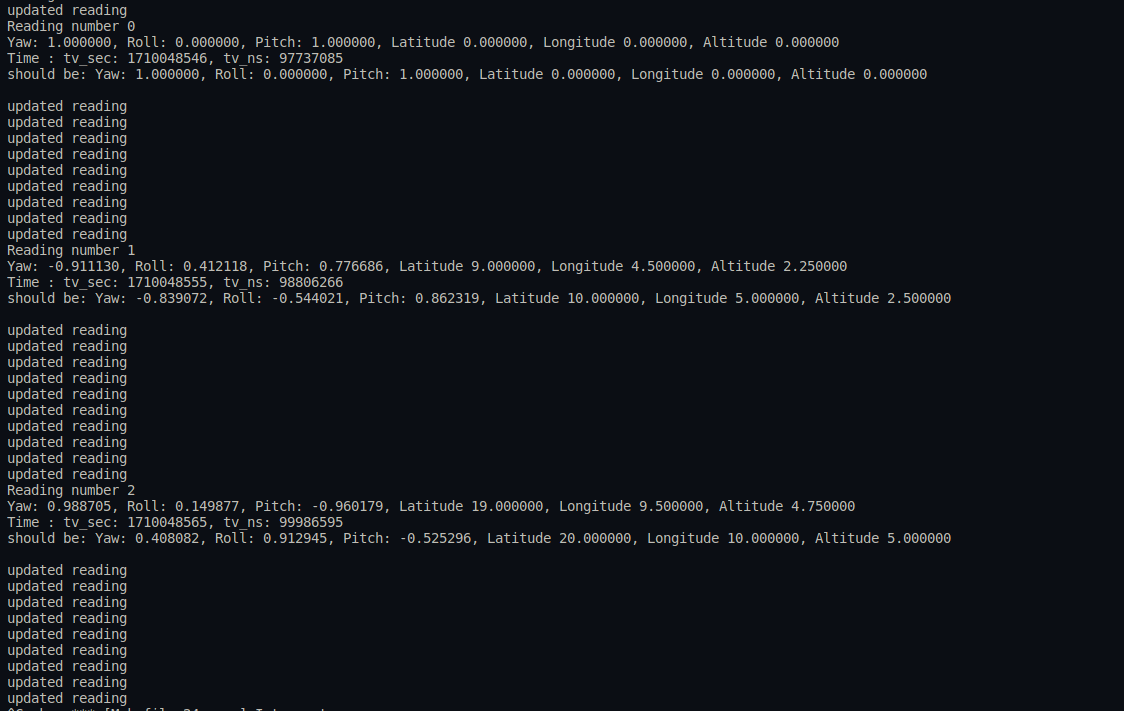
\includegraphics[scale=0.45]{figures/simple.png}
						\caption{Output of simple mutex synchronization}
					\end{figure}

					  Code is given in separated folder (Code\_Q2\_5/2c/simple.c)and in the appendices.

			\end{enumerate}


	\end{enumerate}




	\section{Question 3}
	\begin{enumerate}
		\item[] \Q [20 points] Download example-sync-updated-2/ and review, build, and run it.
			\begin{enumerate}
				\item \Q Describe both the issues of deadlock and unbounded priority inversion and the root cause
				      for both in the example code.
				      \A Deadlock occurs when threads or processes are stuck waiting for each other to release resources they need. For instance, if thread 1 holds resource A and waits for B, while thread 2 holds B and waits for A, they're stuck. \\
				      Following are the outputs and root cause for the example codes:\\

					  \begin{figure}[H]
						\centering
						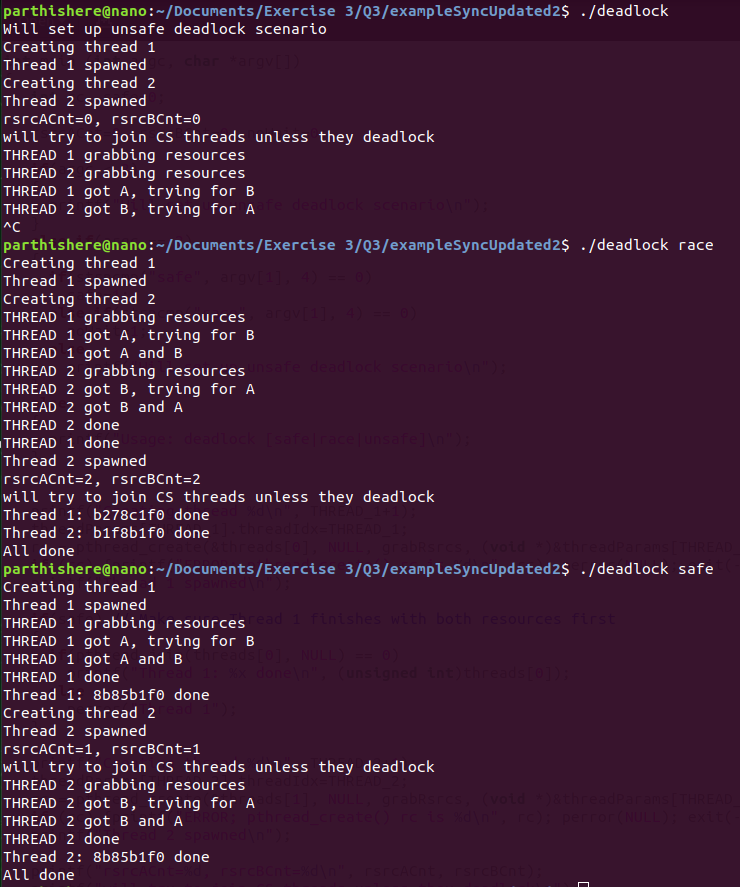
\includegraphics[scale=0.6]{figures/deadlock1.png}
						\caption{Deadlock.c}
					\end{figure}

				      The deadlock.c code can be run in 3 different ways:\\
				      \begin{enumerate}
					      \item \textbf{Without any argument - ./deadlock}\\
					            This scenario depicts the actual deadlock where 2 threads are accessing the same function “grabRsrcs”. Thread 1 acquires the lock “rsrcA” and sleeps for 1 second. Thread 2 acquires the lock “rsrcB” and sleeps for 1 second. Next, when thread 1 tries to acquire “rsrcB” and thread 2 tries to acquire “rsrcA”, a deadlock situation is created as the lock required by one thread is already acquired by the other thread. Referring to the first portion of image, we can observe that since the deadlock has occurred, the code is stuck as both threads are waiting for the locks.

					      \item \textbf{./deadlock race}\\
					            When race is used as an argument, a variable “noWait” is set to 1 which results in both threads not waiting for 1 second after acquiring their respective first lock. This results in one thread completing and releasing both locks before the other thread requires the lock. The code doesn’t create a deadlock but creates a race condition where any thread could execute any time and update the variables “rsrcACnt” and “rsrcBCnt” in a way which is not expected. The execution and values of variables are not fixed each time the code runs and hence the output is unpredictable. Since the threads are not blocking the resource, chances of a deadlock occurring are minimal but still can be possible.

					      \item \textbf{./deadlock safe}\\
					            As observed in the last portion of the image, thread 1 executes first before thread 2 is created. In the code, when safe is passed as an argument, the “safe” variable is set to 1 which waits for the thread 1 to complete first before creating thread 2 and waiting for thread 2 to complete. In this way, the threads don’t run in parallel, avoiding the deadlock scenario.

								\begin{figure}[H]
									\centering
									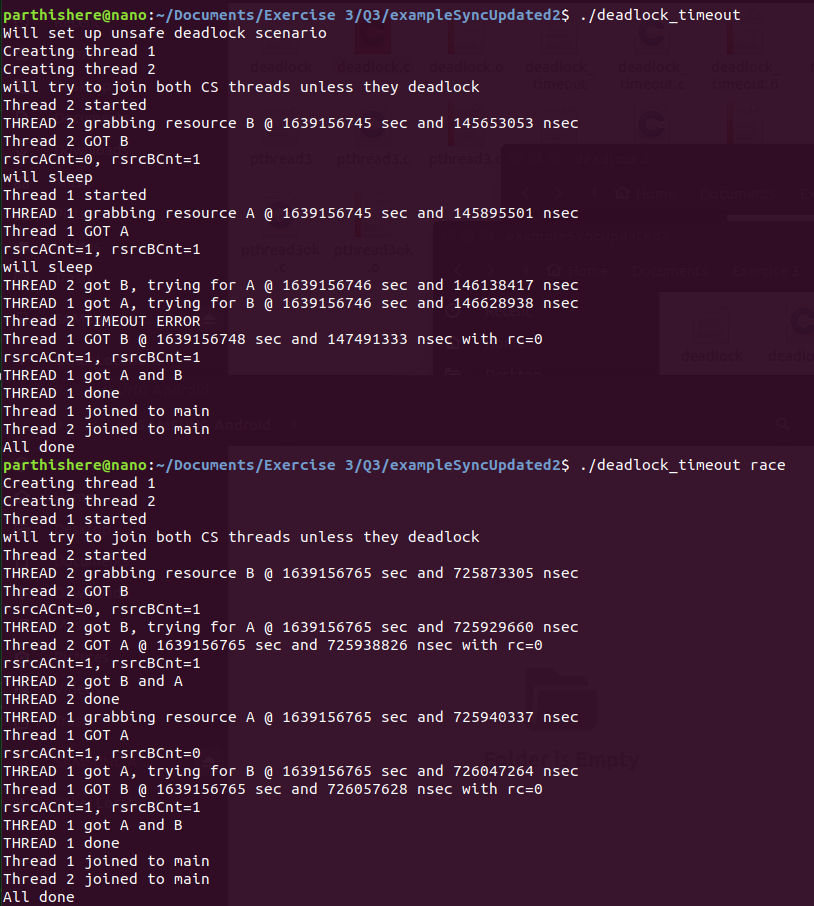
\includegraphics[scale=0.6]{figures/deadlock_timeout.png}
									\caption{Deadlock\_timeout.c}
								\end{figure}

								\begin{figure}[H]
									\centering
									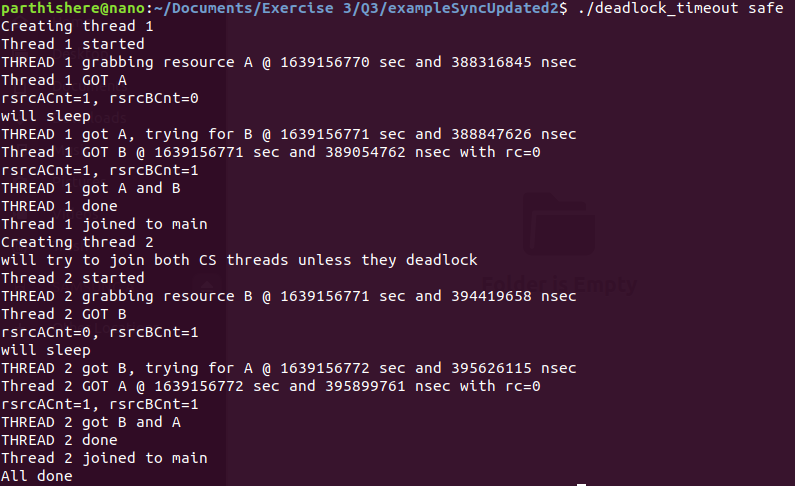
\includegraphics[scale=0.6]{figures/timeout_safe.png}
									\caption{Deadlock\_timeout.c with different parameter}
								\end{figure}

					            Like deadlock.c, the deadlock\_timeout code can run in 3 different ways. The race and safe conditions are the same as deadlock.c and can be referred to in that section.\\
					            In deadlock\_timeout.c, both the threads acquire their first locks – thread 1 acquires “rsrcA“ and thread 2 acquires “rsrcB”. However, both the threads have a timeout before acquiring the second lock (using “pthread\_mutex\_timedlock()”). This timeout is around 3 seconds from the current time obtained from clock\_gettime with CLOCK\_REALTIME. In the first portion of the image, we can observe that both the threads have acquired the first lock but are waiting for the second lock. However, thread 2 is not able to acquire the second lock before the timeout which results in it releasing its first lock and exiting which can be seen by “Thread 2 TIMEOUT ERROR” in the code output. Soon after this, thread 1 acquires the second lock and executes the remaining code. In this case, thread 1 is completely executing but thread 2 doesn’t because of a timeout error in acquiring the second lock.\\\\

					            \textbf{Priority inversion} happens when a high-priority task must wait for a low-priority task to finish using a resource it needs. If the low-priority task gets interrupted by another high-priority task, the high-priority task must wait even longer until the low-priority task finishes. This delay is called bounded priority inversion, and we can plan for it by adding extra time to the schedule to make sure everything gets done on time. But if a medium-priority task comes along and interrupts the low-priority task, we can't predict how long it will take or how many times it will happen. This unpredictable delay is called unbounded priority inversion.\\\\
					            Following are the outputs and root cause for the example codes:




					            \textbf{pthread3.c}
								\begin{figure}[H]
									\centering
									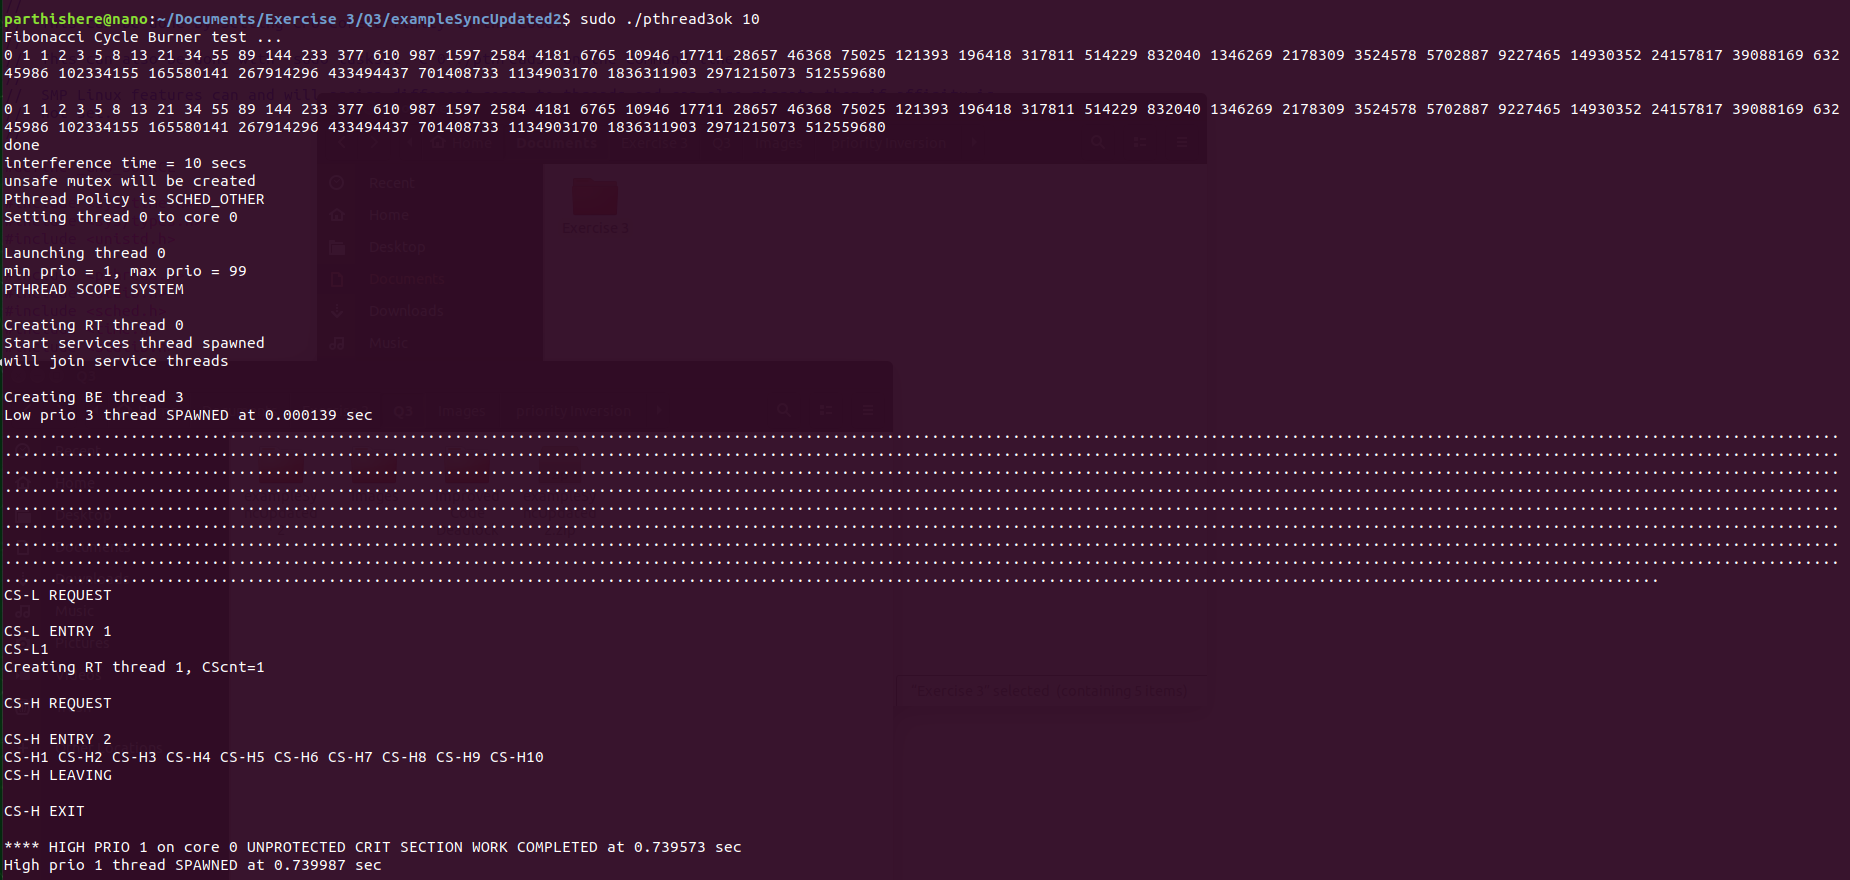
\includegraphics[scale=0.37]{figures/pthread3ok.png}
									\caption{pthread3.c}
								\end{figure}

								\begin{figure}[H]
									\centering
									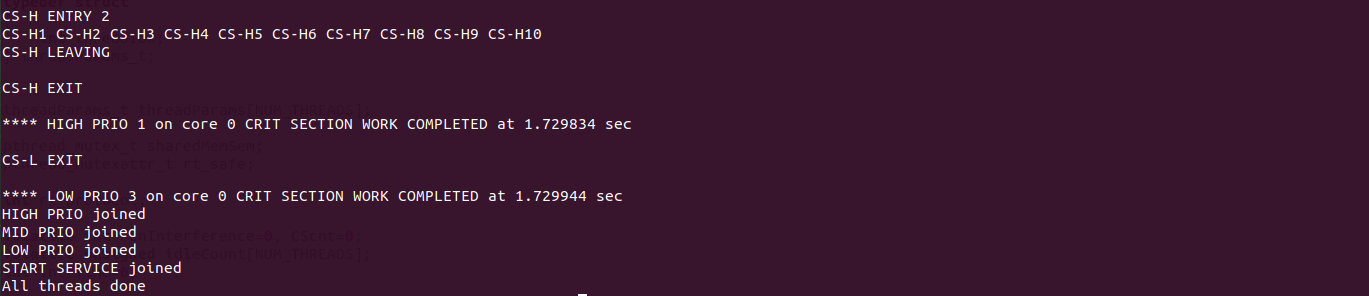
\includegraphics[scale=0.45]{figures/i.png}
									\caption{pthread3.c}
								\end{figure}

					            This code is run with argument 10 which provides the input for interference time. The code has 4 threads – High, mid and low priority threads, and a service thread which schedules their execution. All the threads have their CPU affinity set to the same core. After the service thread, high priority as the name suggests is the highest priority thread followed by mid and low priority threads. Ideally, the highest priority should complete its execution first, followed by mid and then low. In the “startService” function executed by the service thread, the lowest priority thread is created first which enters the critical section in the “criticalSectionTask” function. To ensure that the lowest priority thread enters the critical section, there is a loop in “startService” function which delays the code till the lowest priority thread acquires the lock. The highest priority thread is created next which also executes the “criticalSectionTask” function but is unable to acquire the lock as the lowest priority thread has the lock and hasn’t been able to release it. Next, the mid priority thread is created which executes the “simpleTask” function which doesn’t have a critical section and executes the Fibonacci series based on the interference time entered as an argument. Since the highest priority is blocked due to unavailability of the resource, the mid priority runs the Fibonacci series 10 times (As seen by “M1 M2 ……. M10” in the image) after which the lowest priority runs the Fibonacci series 10 times as “CS\_LENGTH” is 10 (As seen by CS-L1 CS-L2 …….CS-L10). In the end, the highest priority thread acquires the lock and runs the Fibonacci series 10 times (As seen by CS-H1 CS-H2 …….CS\_H10). This is the unbounded priority inversion where lowest priority thread acquires the lock when it is needed by the highest priority thread and mid priority thread completes its execution which causes further delay.\\\\
					            \textbf{pthread3amp.c}
								\begin{figure}[H]
									\centering
									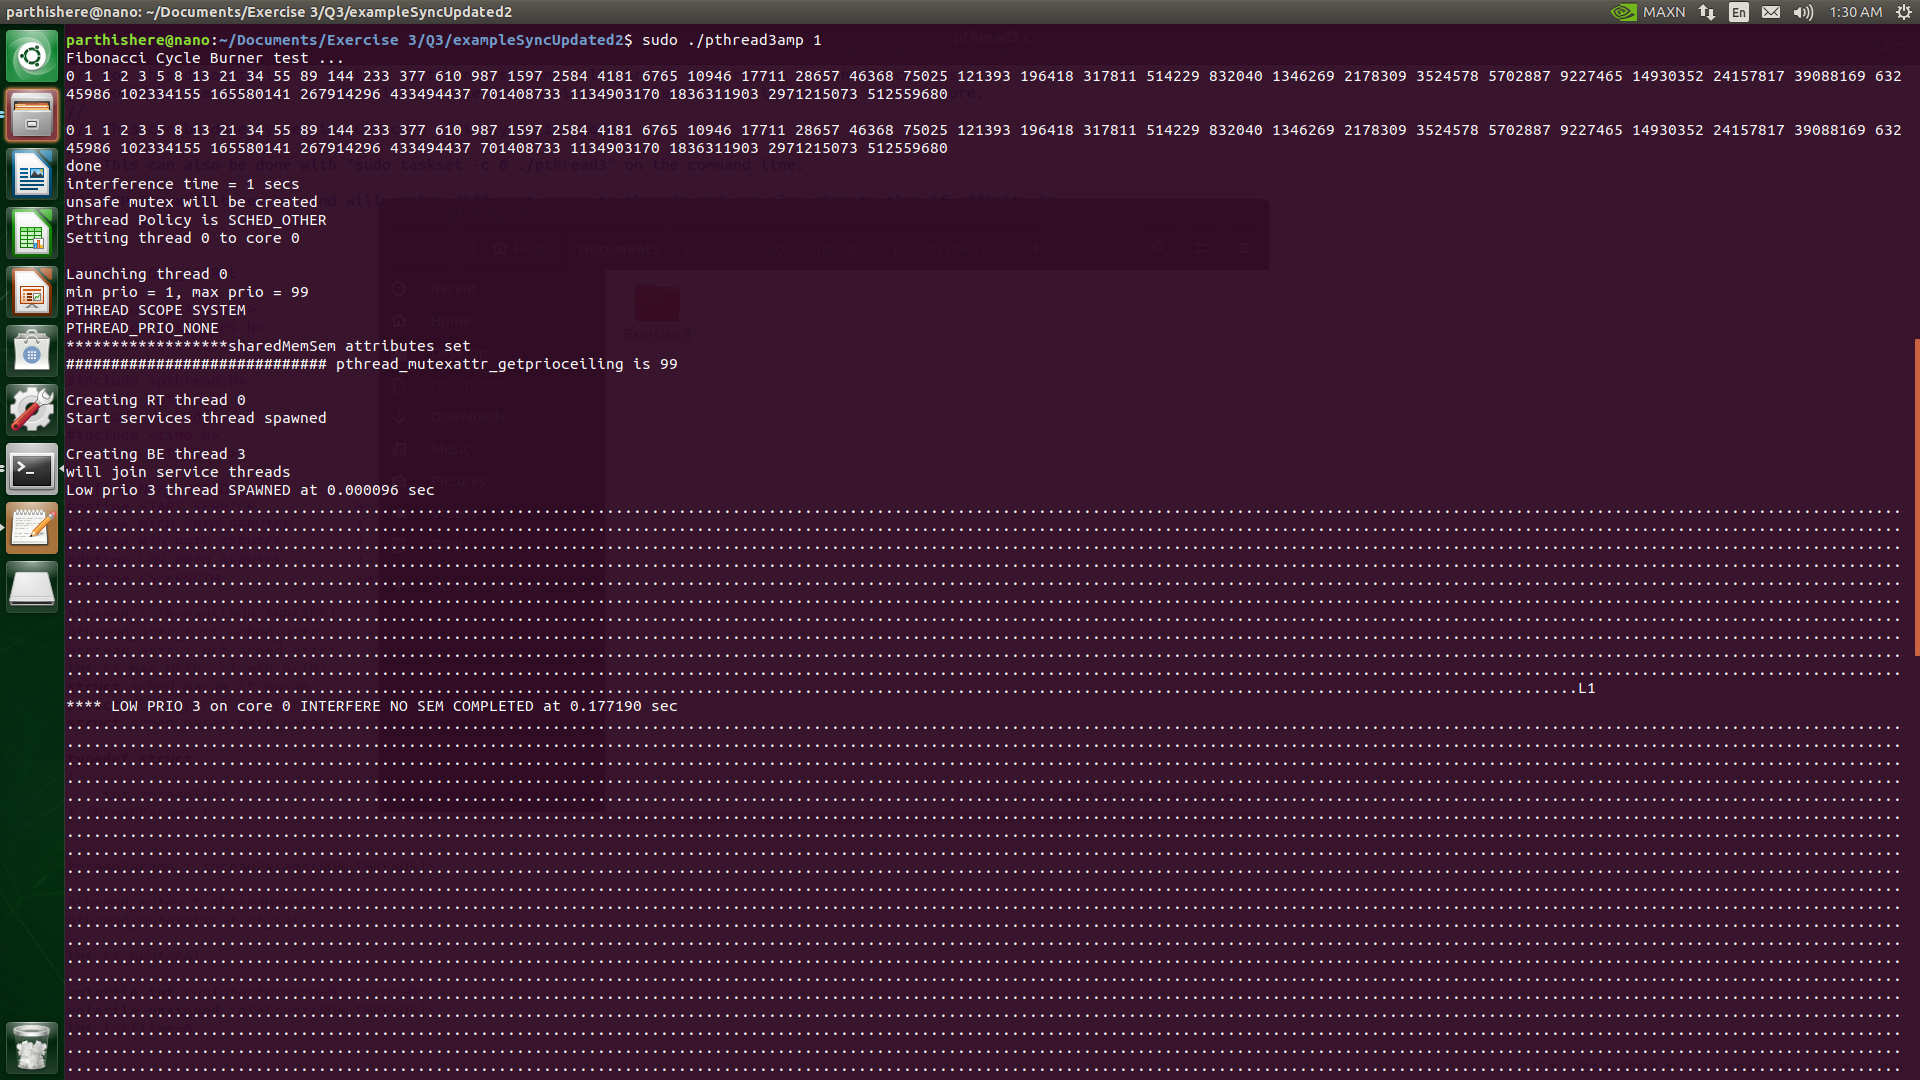
\includegraphics[scale=0.3]{figures/pthread3amp.png}
									\caption{pthread3amp.c}
								\end{figure}
					            This code is like pthread3.c except in this case, the lowest priority thread executes the “simpleTask” instead of the “criticalSectionTask” function. This would ideally avoid the condition for the unbounded priority inversion. But somehow, in the code, inside the “startService” function, the loop to ensure the lowest priority thread enters the critical section and acquires the lock in “criticalSectionTask” function still exists which causes an infinite spin lock. We can observe from the image that when interference time is set to 1, the lower priority thread executes the Fibonacci series once (L1), but the loop continues indefinitely as indicated by the “………”. Hence, no other thread executes.\\\\
					            \textbf{pthread3ok.c}
								\begin{figure}[H]
									\centering
									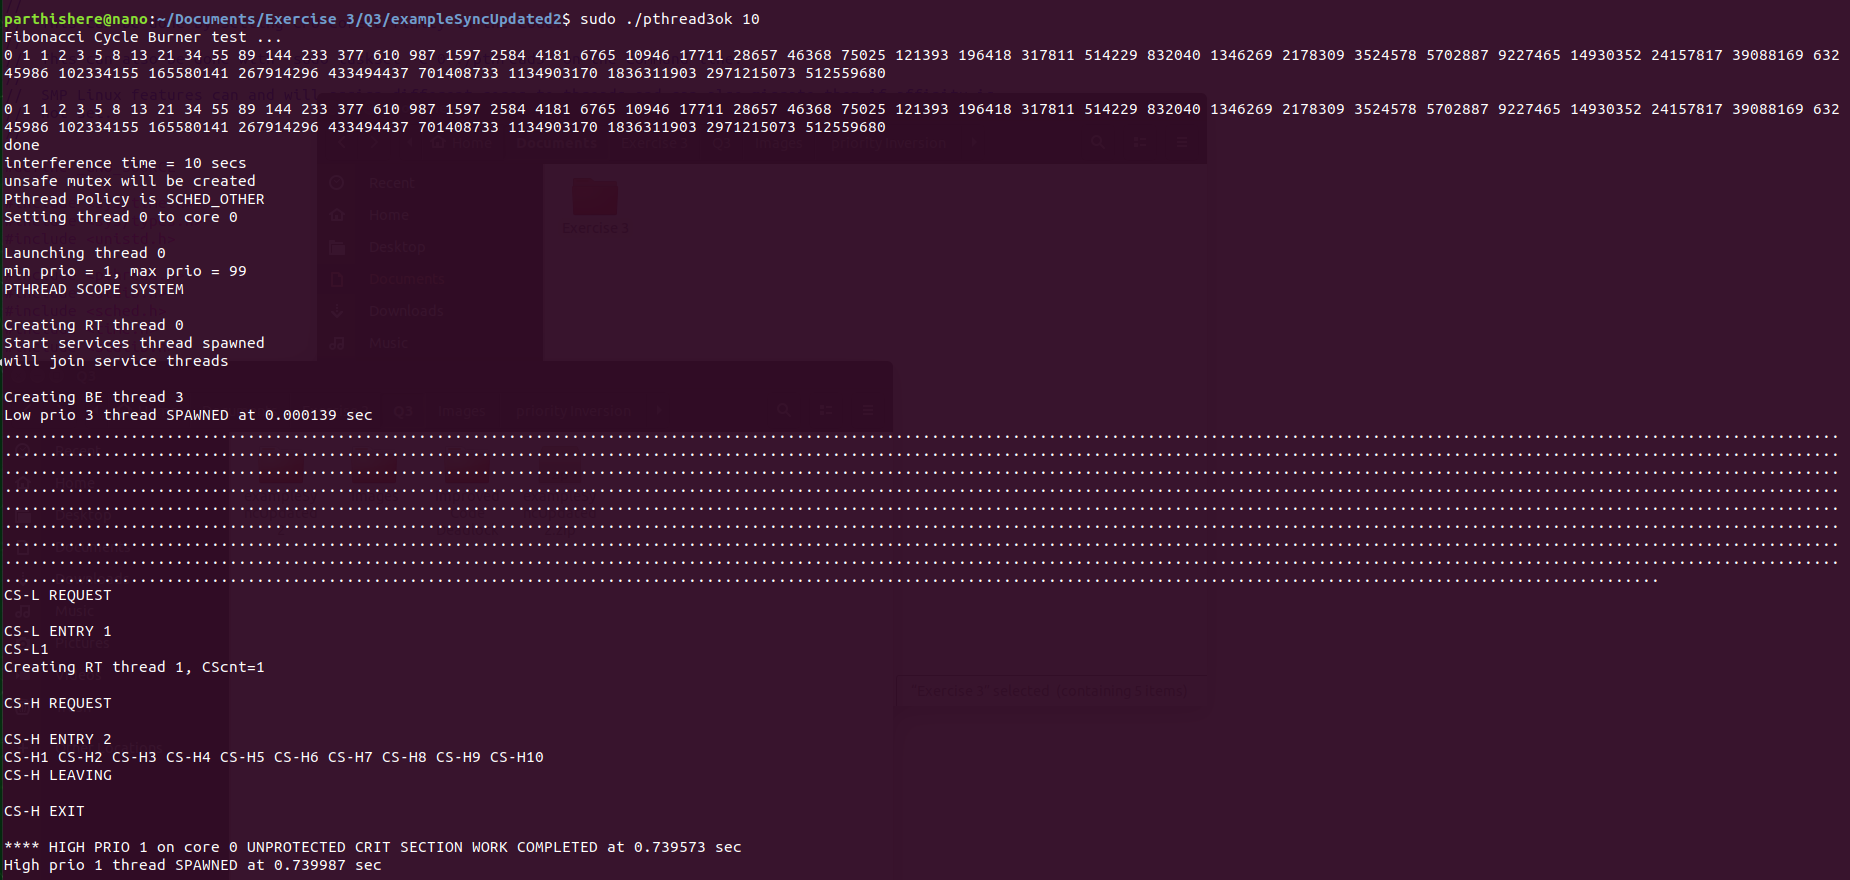
\includegraphics[scale=0.6]{figures/pthread3ok.png}
									\caption{pthread3ok.c}
								\end{figure}

								\begin{figure}[H]
									\centering
									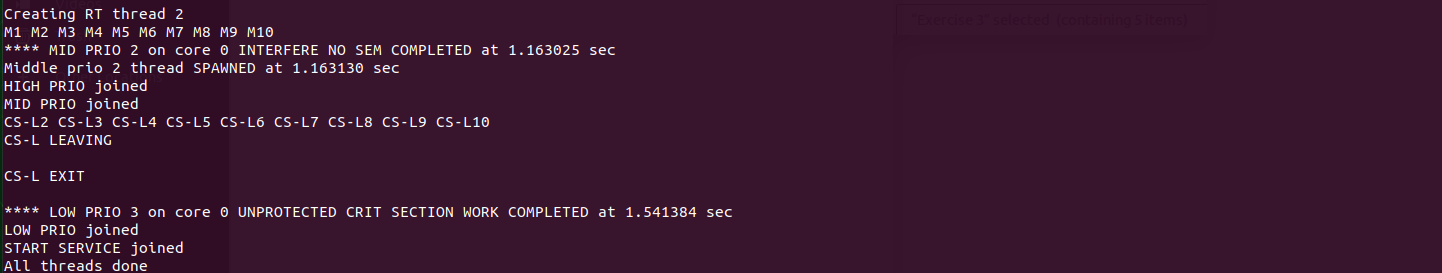
\includegraphics[scale=0.6]{figures/pthread3ok_output.png}
									\caption{pthread3ok.c}
								\end{figure}
					            This code is similar to pthread3.c but it solves the problem of unbounded priority inversion by a method which is not the best solution. As observed from the image, we can confirm that the highest priority thread executes first, followed by the mid priority and in the end lowest priority thread. The fix in the code was that in the “criticalSectionTask” function, the critical section was removed by uncommenting the mutex lock and unlock. In this way, the highest priority thread would preempt the lowest priority thread. This is not an advisable solution for unbounded priority inversion as the critical section needs to be protected and if not, it can lead to sequence and data corruption.\\\\
					            To prevent deadlock, we can set a time limit for holding resources. But if both threads release resources simultaneously, it could lead to another problem called live-lock. To avoid this, we use a random back-off scheme, causing one thread to release a resource while the other holds onto both, breaking the deadlock. The output of the updated deadlock.c can be found below:
								\begin{figure}[H]
									\centering
									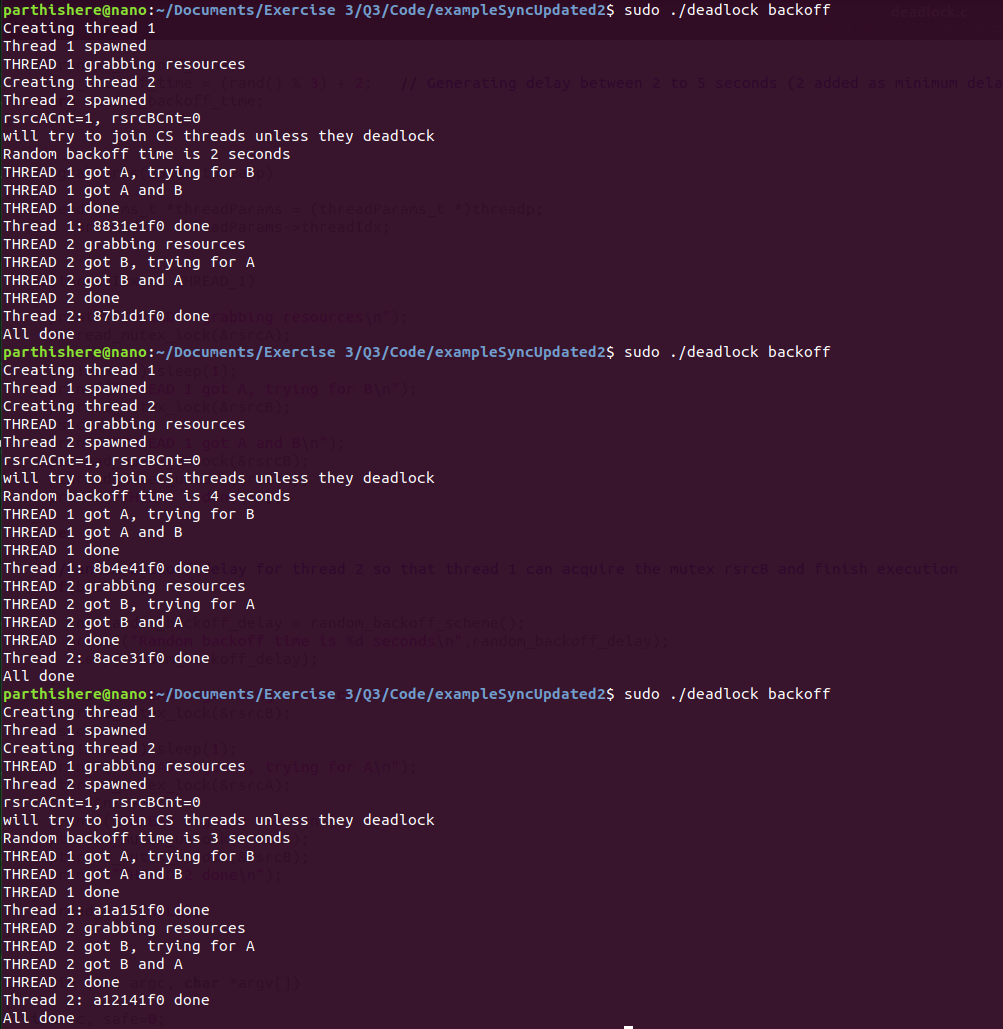
\includegraphics[scale=0.6]{figures/deadlock.png}
									\caption{deadlock.c}
								\end{figure}
								The code was updated to add a random backoff scheme to avoid the deadlock scenario. In the code, a new argument “backoff” was added which would prevent the deadlock using random backoff scheme. A new function “random\_backoff\_scheme” was created which would return a random delay in seconds (between 2 to 5). A rand() function was used to generate a random number which was divided by 3 and the remainder was added to 2. These numbers, minimum range and the delay were calculated using various random combinations in which deadlock wouldn’t occur.  In the “grabRsrcs”, before the thread 2 execution started, this delay was introduced so that thread 1 could execute completely acquiring both the locks and by the time thread 2 executes, both the locks would be available. As observed from the image, thread 1 executes first and then thread 2. The random backoff time for which thread 2 sleeps is also printed. The code was run multiple times and deadlock was not observed.


				      \end{enumerate}


				\item \Q Fix the deadlock so that it does not occur by using a random back-off scheme to resolve.
				      For the unbounded inversion, is there a real fix in Linux – if not, why not?
				      \A \textbf{No, there isn't a fix for unbounded priority inversion in Linux without the RT\_PREEMPT\_PATCH.} This patch, now part of the Linux kernel, supports priority inheritance. Without it, Linux lacks a mechanism to adjust the priority of system calls, leaving unbounded priority inversion unresolved.

				\item \Q What about a patch for the Linux kernel? For example, Linux Kernel.org recommends
				      the RT\_PREEMPT Patch, also discussed by the Linux Foundation Realtime Start and this
				      blog, but would this really help? Read about the patch and describe why think it would
				      or would not help with unbounded priority inversion. Based on inversion, does it make
				      sense to simply switch to an RTOS and not use Linux at all for both HRT and SRT
				      services?
				      \A The RT\_PREEMPT\_PATCH for the Linux kernel turns the kernel space into a preemptible environment like user space. This means that higher priority tasks can be executed immediately, with a few exceptions. It's especially useful for real-time applications. However, it's crucial to handle CPU variables carefully because the kernel isn't preemptible during certain operations like handling interrupts or holding locks.\\\\
					  This patch allows setting priorities for system calls and interrupts. It introduces the concept of priority inheritance to prevent unbounded priority inversion. When a low-priority task is preempted by a higher-priority task, its priority is temporarily raised to ensure the critical section is executed promptly. This strategy converts unbounded priority inversion to bounded, manageable inversion, improving task scheduling reliability.
					  While the RT\_PREEMPT\_PATCH doesn't guarantee the complete elimination of priority inversion, it significantly reduces the risk, making sure unbounded priority inversion won't occur. It empowers users to adjust thread priorities, enhancing system responsiveness and predictability.\\\\
					  Moreover, this patch enables preempting kernel locks, critical sections, and interrupts, further mitigating priority inversion. By utilizing priority inheritance, it minimizes the blocking time of high-priority tasks, contributing to the development of robust real-time systems.\\\\
					  
					  However, there are some limitations. For instance, if a low-priority thread inherits a high priority for an extended period, it may impact system performance. Despite these challenges, the RT\_PREEMPT\_PATCH effectively addresses and resolves the problem of unbounded priority inversion, improving the reliability of real-time systems built on the Linux kernel.
					  Based on inversion, does it make sense to simply switch to an RTOS and not use Linux at all for both HRT and SRT services?
					  Ans. Switching from Linux to an RTOS depends on the application's needs. Linux, with its extensive codebase and community support, isn't optimized for real-time tasks. Even with enhancements like the RT\_PREEMPT\_PATCH, Linux may struggle with priority inversion, where higher-priority tasks are delayed by lower-priority ones, affecting hard real-time applications.
					  In contrast, RTOS is purpose-built for real-time tasks and typically handles priority inversion more effectively. This makes it suitable for projects with strict real-time requirements, especially those where developing code from scratch is feasible. RTOS provides the precise timing and reliability crucial for hard real-time systems.\\\\
					  However, Linux has its strengths, such as an excessive number of tools and existing code, making it popular for many applications. While Linux, with the RT\_PREEMPT\_PATCH, can handle soft real-time tasks well, relying solely on it for hard real-time services may pose challenges.\\\\
					  Additionally, the architecture and design of the Linux kernel impact its real-time capabilities. While patches like RT\_PREEMPT\_PATCH aim to enhance real-time performance, they may not fully resolve all issues, particularly in situations requiring strict real-time guarantees. Thus, for applications needing precise real-time performance, an RTOS may provide a more reliable solution.\\\\
					  The decision to switch to an RTOS depends on various factors, including the criticality of real-time requirements, available resources, and project specifics. While Linux, with appropriate patches, can address some real-time concerns, an RTOS remains the preferred choice for hard real-time services due to its specialized architecture and reliability.
			\end{enumerate}


	\end{enumerate}

	\pagebreak
	\section{Question 4}
	\begin{enumerate}
		\item[] \Q [15 points] Review POSIX-examples and especially POSIX\_MQ\_LOOP and build the code
			related to POSIX message queues and run them to learn about basic use.
			\begin{enumerate}
				\addcontentsline{toc}{subsection}{A}
				\item \Q  First, re-write the simple message queue demonstration code in heap\_mq.c and
				      posix\_mq.c so that it uses RT-Linux Pthreads (FIFO) instead of SCHEDULE\_OTHER,
				      and then write a brief paragraph describing how the two message queue applications are
				      similar and how they are different. Prove that you got the POSIX message queue features
				      working in Linux on your target board.
				      \A The code in VxWorks provided by Sam Siewert was ported to RT-Linux Pthreads. For both heap\_mq.c and posix\_mq.c, 2 threads were created : sender and receiver where both were scheduled with SCHED\_FIFO policy with the sender given higher priority than receiver. Both these threads were referencing a message queue "/send\_receive\_mq" where sender thread was enqueuing the messages in the message queue till maximum messages and then receiver thread was dequeuing one message from the message queue in an infinite loop. Both the threads were configured to use the same core.\\\\
				      heap\_mq.c output
					  \begin{figure}[H]
						\centering
						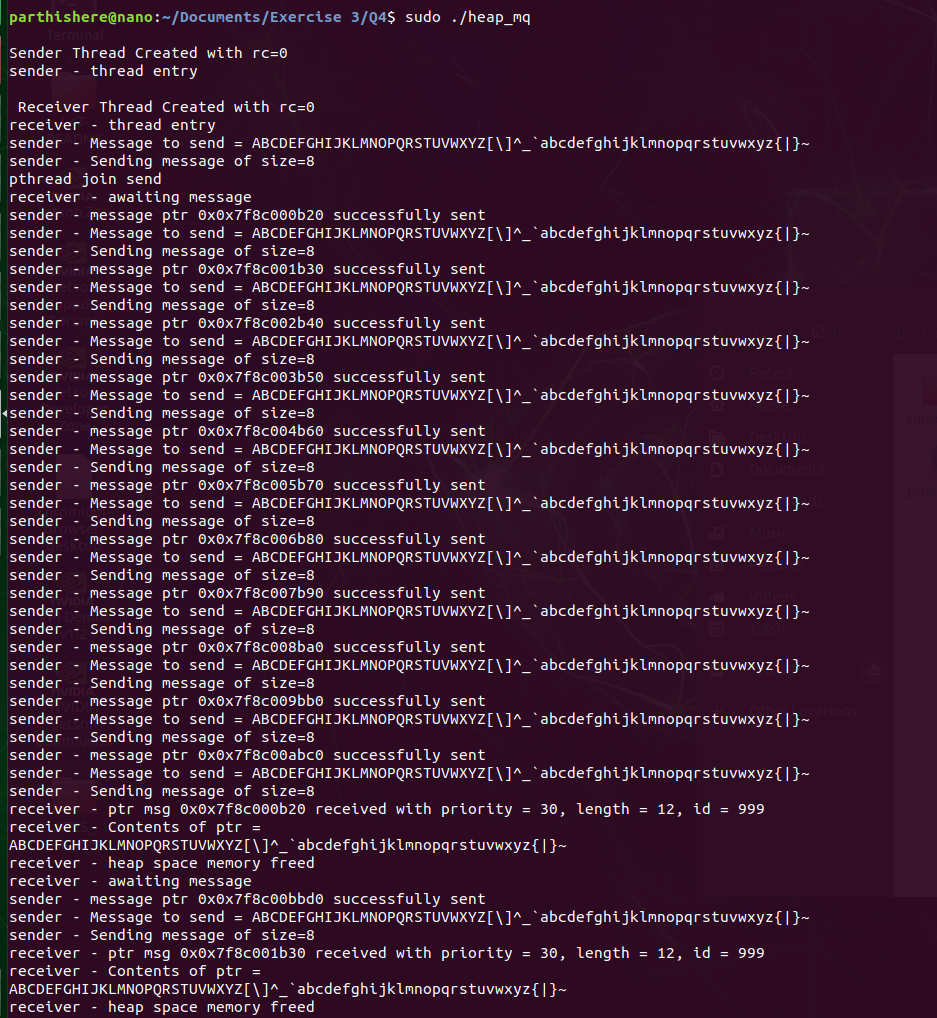
\includegraphics[scale=0.6]{figures/heapmq.png}
						\caption{heapmq.c}
					\end{figure}


				      As observed from the output, the sender has enqueued 10 messages in the message queue (addresses of the heap memory where buffer data is copied) and the heap addresses and data contained in that memory is printed on terminal. The data contains ASCII characters and an id. The receiver thread dequeues the message queue (first-in message) to obtain the address. This address is copied to a local buffer which is then dereferenced to obtain the ASCII characters and id. From the prints, we can confirm the addresses enqueued by sender thread and dequeued by receiver thread are same and the data pointed by those addresses are same as well. After one message is dequeued, since the sender thread has a higher priority, it preempts the receiver thread and enqueues one more message before going into blocking state where receiver thread then dequeues the next in line message in the message queue.
				      posix\_mq.c output\\\\
					  \begin{figure}[H]
						\centering
						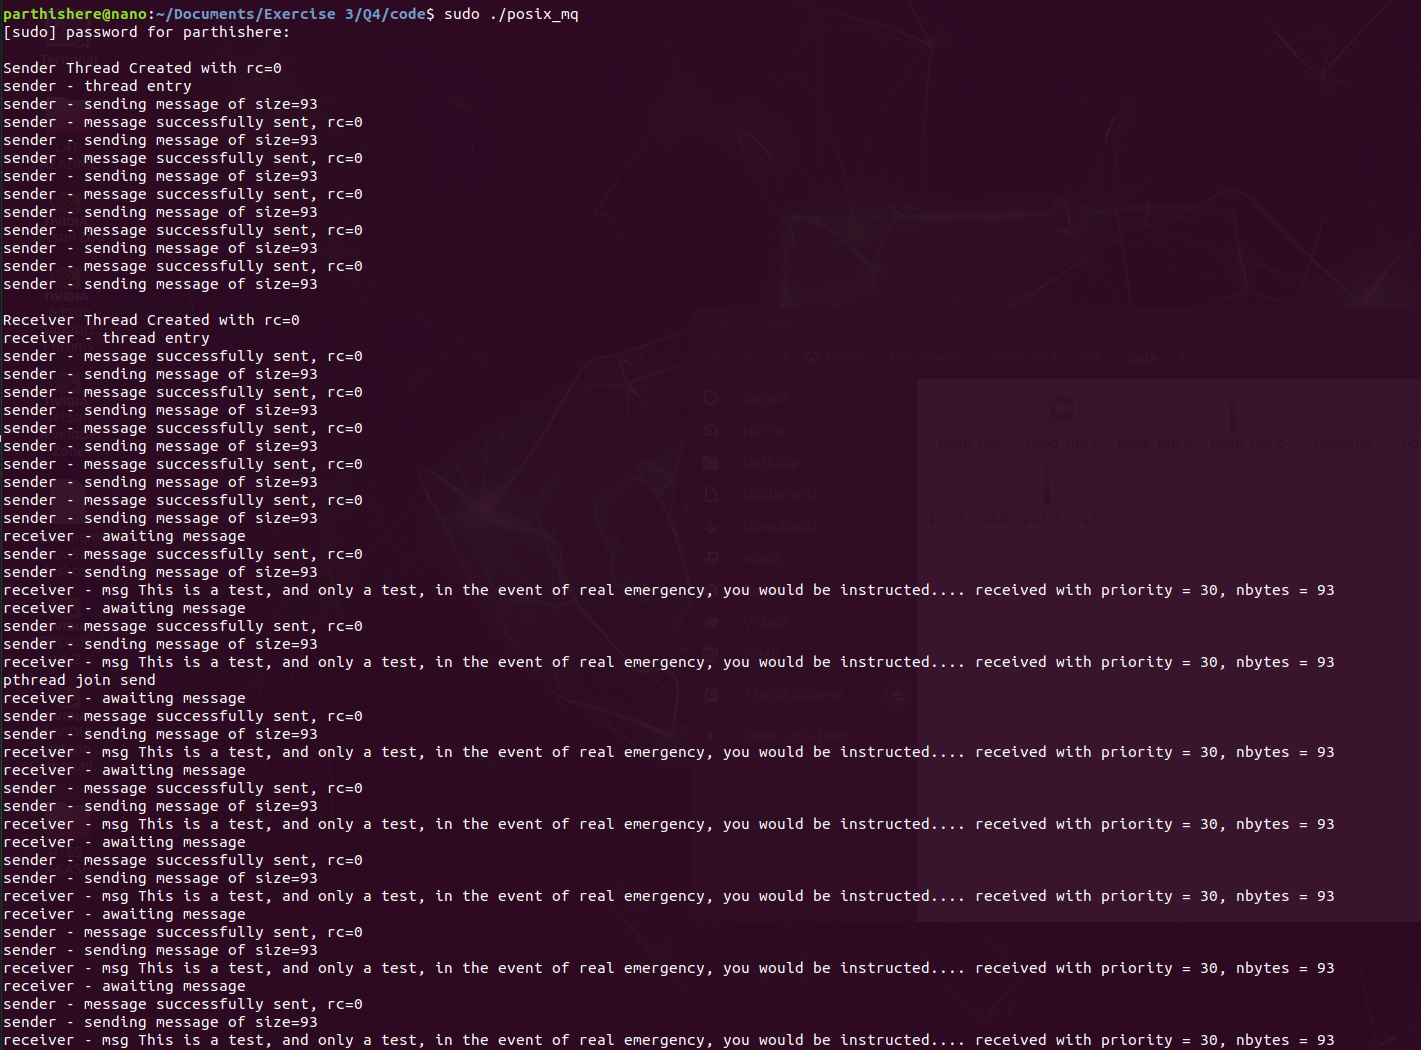
\includegraphics[scale=0.6]{figures/posix_mq.png}
						\caption{posix\_mq.c}
					\end{figure}

				      Observing the output, the sender has enqueued 10 messages in the message queue (string of fixed size) verified with a print of number of bytes transferred. The receiver thread dequeues the message queue (first-in message) to obtain the address. This address is copied to a local buffer which is then printed as a string. From the prints, we can confirm the string sent by the sender thread and received by the receiver thread are same. After one message is dequeued, since the sender thread has a higher priority, it preempts the receiver thread and enqueues one more message before going into blocking state where receiver thread then dequeues the next in line message in the message queue.
				      Code for heap\_mq.c can be found in Appendix 1 and code for posix\_mq.c can be found in Appendix 2.

				      Similarities between both codes
				      \begin{enumerate}
					      \item Both the codes have 2 threads – sender and receiver which access the same message queue.
					      \item Both codes work as expected – The sender enqueues messages in the queue whereas the receiver dequeues the messages. In both cases, the message sent by sender and received by receiver are the same.
					      \item  In both cases, the sender enqueues 10 messages (max number of messages that can be enqueued in message queue) before going into blocking state after which receiver thread executes and dequeues the first in message in the message queue after which the sender thread preempts the receiver thread.
					            Differences between both codes
					      \item In posix\_mq.c, the actual data is transferred between the two threads through the message queue. In this case, the data has a restriction to be under the maximum size mentioned in the message queue attributes. In heap\_mq.c, the address of the heap is passed instead of actual data. In this case, there is no restriction on the size of the data as the message queue will only contain the address. The receiver thread can dereference the heap address to obtain the data.
					      \item In posix\_mq.c, the buffered message is stored as a static i.e. it is stored in the data segment of the memory whereas in heap\_mq.c, the data is stored in heap. The heap is shared by both threads, the sender thread allocates the memory (by malloc) whereas the receiver thread frees the memory after reading the data in it.
				      \end{enumerate}

				      \addcontentsline{toc}{subsection}{B}
				\item \Q Message queues are often suggested as a way to avoid MUTEX priority inversion.
				      Would you agree that this really circumvents the problem of unbounded inversion? If so
				      why, if not, why not?
				      \A . I would agree that message queues can effectively circumvent the issue of unbounded priority inversion because of the following reasons:
					  \begin{enumerate}
						\item[] Priority Messaging: POSIX message queues have the capability to assign priorities to messages, ensuring that higher priority messages are dequeued before lower priority ones. This means that higher priority tasks don't need to wait indefinitely for lower priority tasks to release resources, thus avoiding unbounded priority inversion.
						\item[] FIFO Logic: If two messages have the same priority, POSIX message queues follow a First-In-First-Out (FIFO) logic. This ensures fairness in message processing and helps prevent scenarios where lower priority tasks in definitely delay higher priority ones.
						\item[] Thread-Safe Operations: Enqueue and dequeue operations on message queues are thread-safe. This means that multiple threads can safely access the queue without causing conflicts or race conditions.
						\item[] Resource Management: Message queues provide a mechanism for threads to synchronize their execution by pausing until a message is available in the queue. This prevents threads from spinning needlessly and consuming CPU resources while waiting for shared resources.
					  \end{enumerate}
				      
				      
				      
				      In summary, message queues, particularly POSIX message queues, address the issues of unbounded priority inversion by providing priority-based message handling and ensuring thread-safe operations. They facilitate efficient communication between threads and help maintain system responsiveness even in scenarios involving shared resources and differing task priorities.

			\end{enumerate}


	\end{enumerate}

	\section{Question 5}
	\begin{enumerate}
		\item[] \Q [20 points] Watchdog timers, timeouts and timer services – First, read this overview of the
			Linux Watchdog Daemon and the Linux manual page on the watchdog daemon -
			https://linux.die.net/man/8/watchdog . Also see the Watchdog Explained.
			\begin{enumerate}
				\addcontentsline{toc}{subsection}{A}
				\item \Q Describe how it might be used if software caused an indefinite deadlock.
				      \A
					  The watchdog utility, as described in the Linux manual, is a daemon that monitors and/or restarts a system if it detects that the system has become unresponsive. It operates by continually kicking (updating) a watchdog timer; if the timer expires (i.e., it is not kicked within a certain period), the system is considered to have failed and is subsequently rebooted. This can be particularly useful in situations where software has caused the system to enter an indefinite deadlock, making it unresponsive.\\\\

					  Using watchdog in the Context of a Deadlock
					  An indefinite deadlock occurs when two or more processes hold resources and each process is waiting for the other to release a resource, causing all processes to be stuck indefinitely. In critical systems, such deadlocks can lead to severe consequences, including loss of data, unavailability of services, and potential hardware damage due to overheating or overuse.\\\\
					  
					  Here’s how watchdog can be utilized to mitigate the impact of such a deadlock:
					  
					  \begin{itemize}
						\item Detection of Unresponsiveness: watchdog is configured to detect system unresponsiveness or failure to execute critical tasks within expected timeframes.
						\item  Heartbeat Mechanism: For software that might cause a deadlock, implementing a heartbeat mechanism that periodically signals watchdog can be an effective strategy. The software must regularly kick the watchdog timer to prevent the system from being rebooted. If the software enters a deadlock and fails to kick the timer, watchdog will reboot the system once the timer expires.
						\item Recovery Actions: Upon detecting a failure (e.g., a timeout indicating a deadlock), watchdog can take predefined actions to recover the system. Typically, this involves rebooting the system to resolve the deadlock and restore service.
					  \end{itemize}
					  
					

				      \addcontentsline{toc}{subsection}{B}
				\item \Q Next, to explore timeouts, use your code from \#2 and create a thread that waits on a
				      MUTEX semaphore for up to 10 seconds and then un-blocks and prints out “No new data
				      available at <time>” and then loops back to wait for a data update again. Use a variant of
				      the pthread\_mutex\_lock called pthread\_mutex\_timedlock to solve this programming
				      problem.
				      \A 

					  \textbf{Data Structures:}
					  \begin{enumerate}
						\item Data Structures:
						\begin{itemize}
							\item NavigationState: Holds navigation-related data (latitude, longitude, altitude, roll, pitch, yaw) and a timestamp.
							\item ThreadArgs\_t: Designed to pass arguments to threads, though not extensively used in the provided snippet.
							\item  RmTask\_t: Contains parameters for configuring threads, including scheduling properties, function pointers for thread routines, thread IDs, and CPU affinity settings.
						\end{itemize}
						\item Global Variables:
						\begin{itemize}
							\item mutex and state\_mutex: Mutexes used for synchronization, although only state\_mutex is utilized for protecting access to nav\_state.
							nav\_state and nav\_state\_shouldbe: Instances of NavigationState for holding current and expected navigation data.
							Thread Functions:
							
							\item update\_thread: Updates nav\_state in a loop with simulated data and timestamps, protected by state\_mutex to ensure exclusive access during updates.
							read\_thread: Attempts to acquire state\_mutex with a timeout using pthread\_mutex\_timedlock and reads nav\_state if successful. It prints a message if it times out, indicating no new data was available for reading.
						\end{itemize}
						

					  \end{enumerate}

					  \textbf{Use of Mutex for Synchronization}\\
The mutex state\_mutex is crucial for ensuring that updates and reads to the shared nav\_state structure are performed atomically, avoiding potential data races. Here's how it's used:

\begin{itemize}
	\item In\ update\_thread: Before updating nav\_state, the thread locks state\_mutex. This ensures that read\_thread cannot simultaneously access nav\_state, potentially reading inconsistent data. After the update, it unlocks state\_mutex, allowing other threads to access nav\_state.
	\item 
	In read\_thread: It tries to lock state\_mutex within a specific timeout period. If successful, it means update\_thread is not currently updating nav\_state, and it can safely read consistent data. If it times out, it indicates that update\_thread has held the lock for too long, suggesting no new data is available for reading within the expected timeframe.	
\end{itemize}



here is the output of the commenting out the 10ms delay so that both tasks are synchronized

\begin{figure}[H]
	\centering
	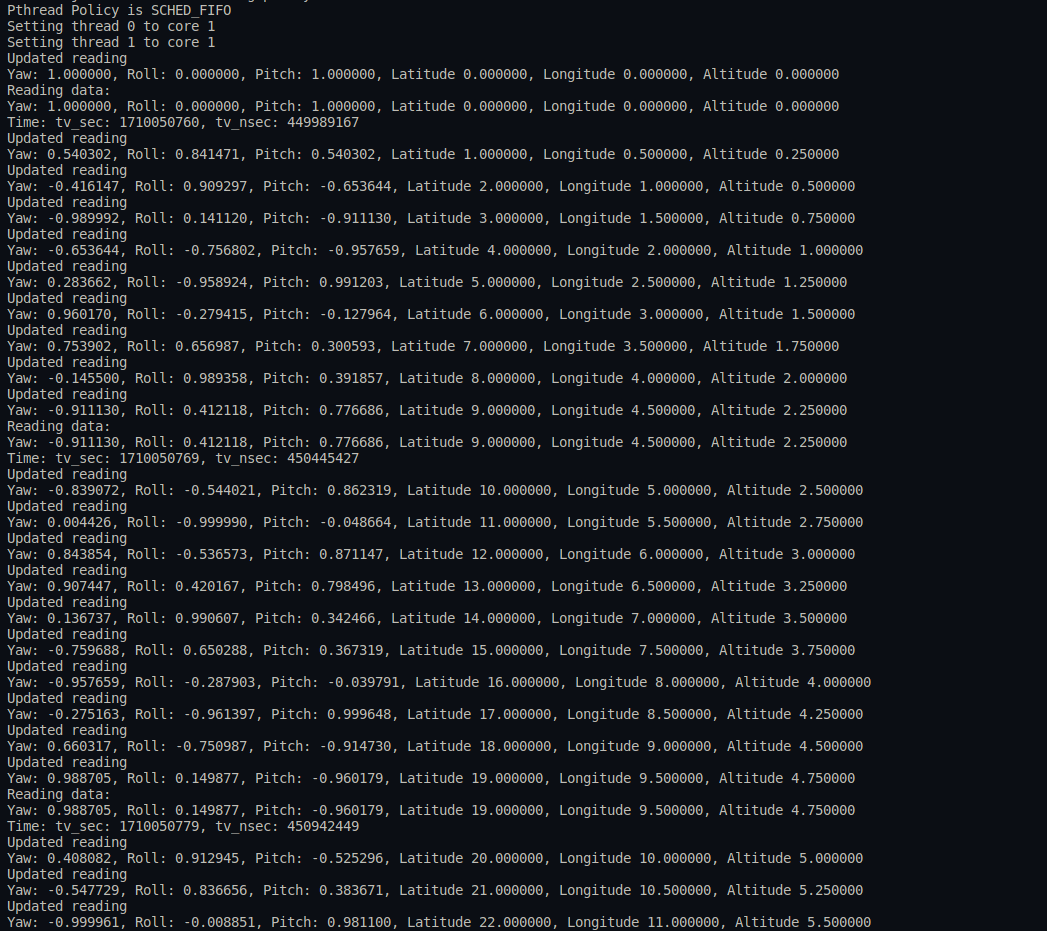
\includegraphics[scale=0.6]{figures/pthread_working.png}
	\caption{Tasks are in synchronization}
\end{figure}


Now enabling 10ms delay while updating tasks so that other task have to wait for the mutex to be unlocked by other task

\begin{figure}[H]
	\centering
	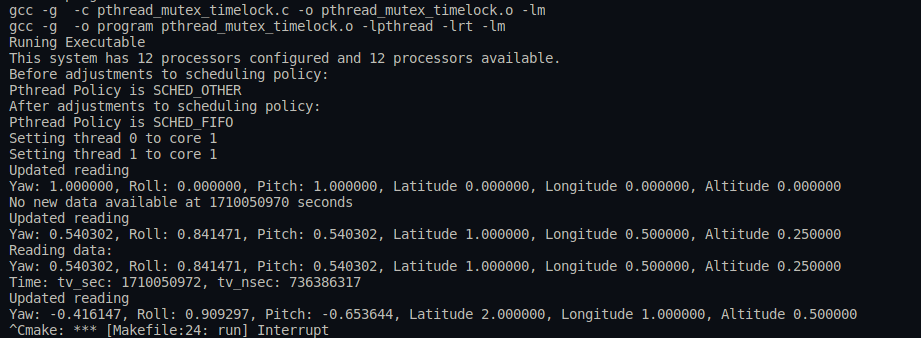
\includegraphics[scale=0.6]{figures/not_working.png}
	\caption{Tasks are not in synchronization}
\end{figure}



			\end{enumerate}

			\section{Question 6}
		\item[] \Q [10 points] Demonstrate the results and answer questions from the TA regarding the code
			you developed in \#2, \#3, \#4, and \#5.
			
	\end{enumerate}

	

	\section{References}
	\begin{enumerate}
		\item ECEN 5623 Lecture slides material and example codes.
		\item REAL-TIME EMBEDDED COMPONENTS AND SYSTEMS with LINUX and RTOS, Sam Siewert John
		      Pratt (Chapter 6, 7 \& 8).
		\item Exercise 3 requirements included links and documentation.
	\end{enumerate}


\end{qanda}




\vfill
\hrule
\vspace{0.5cm}
\pagebreak
\begin{appendices}
	\section{C Code for the Implementation}

	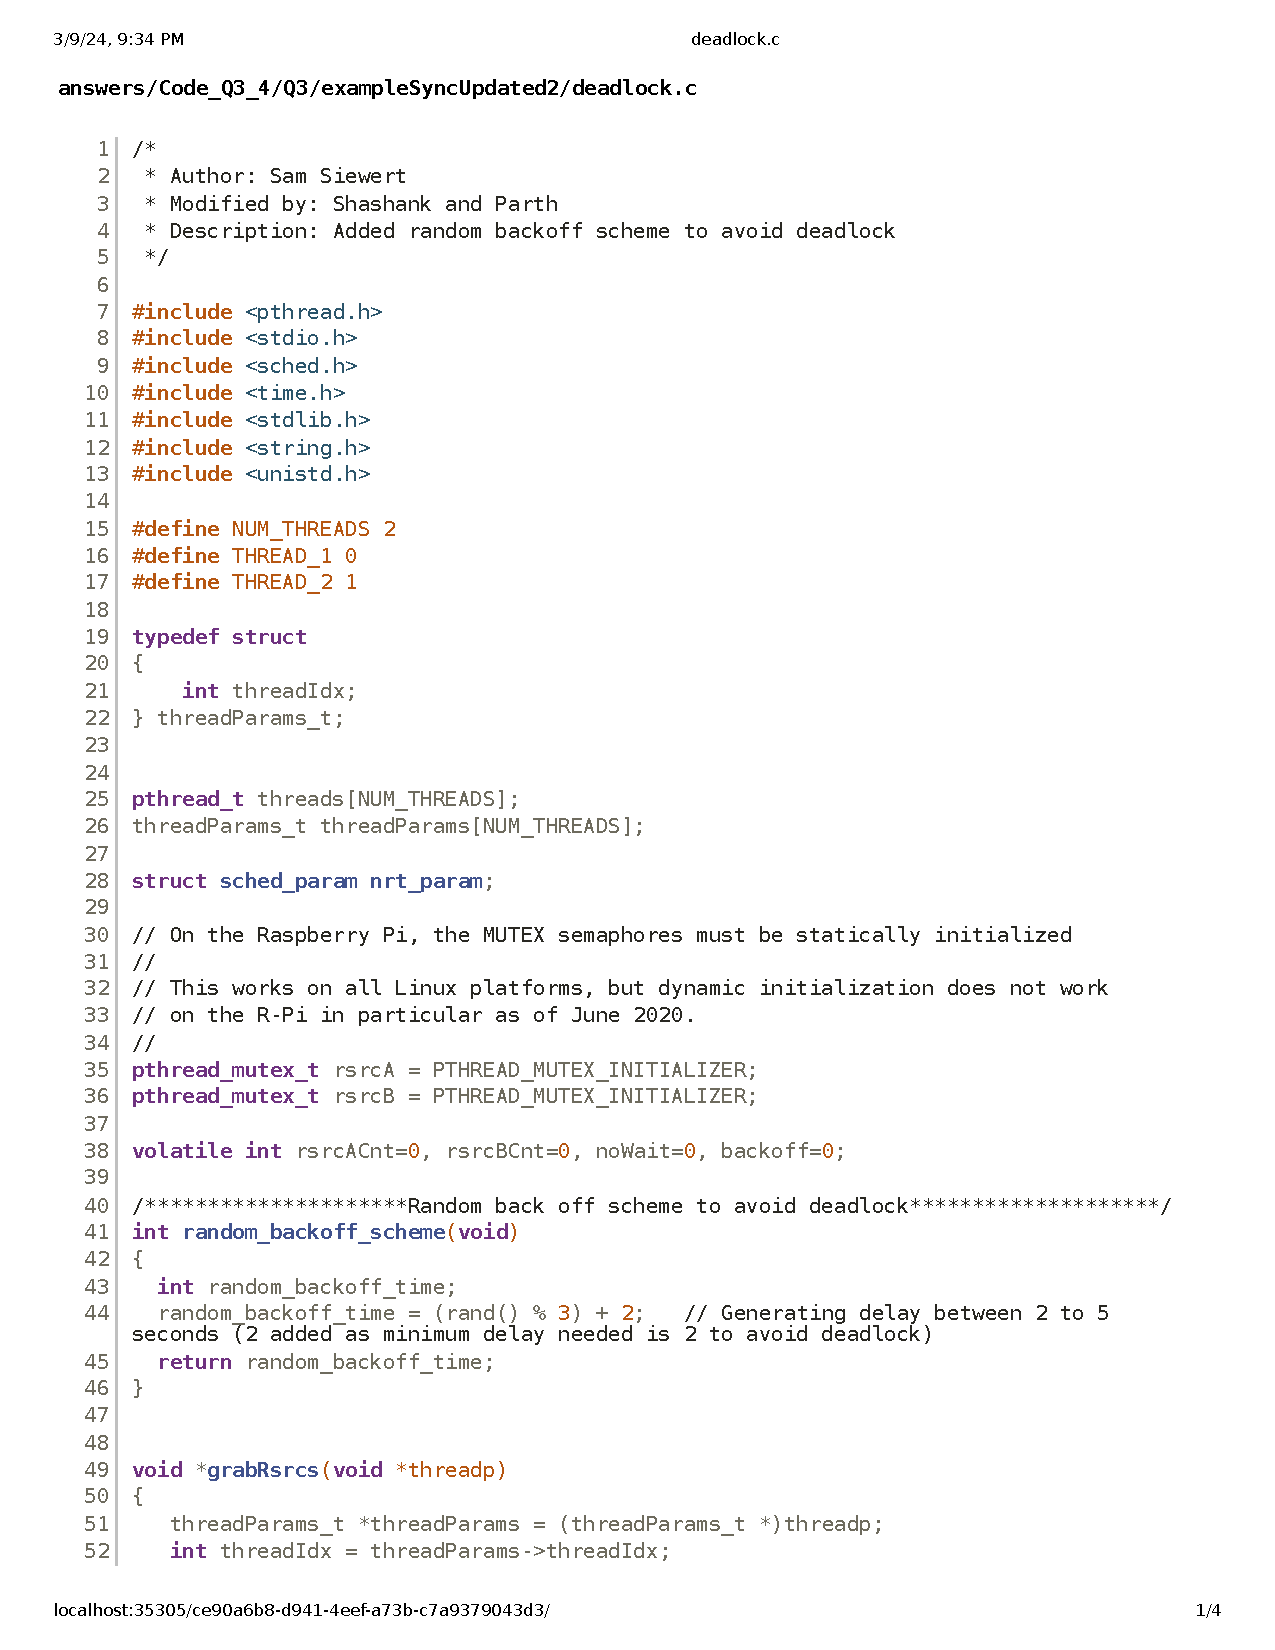
\includepdf[pages=-]{code/deadlock.c.pdf}
	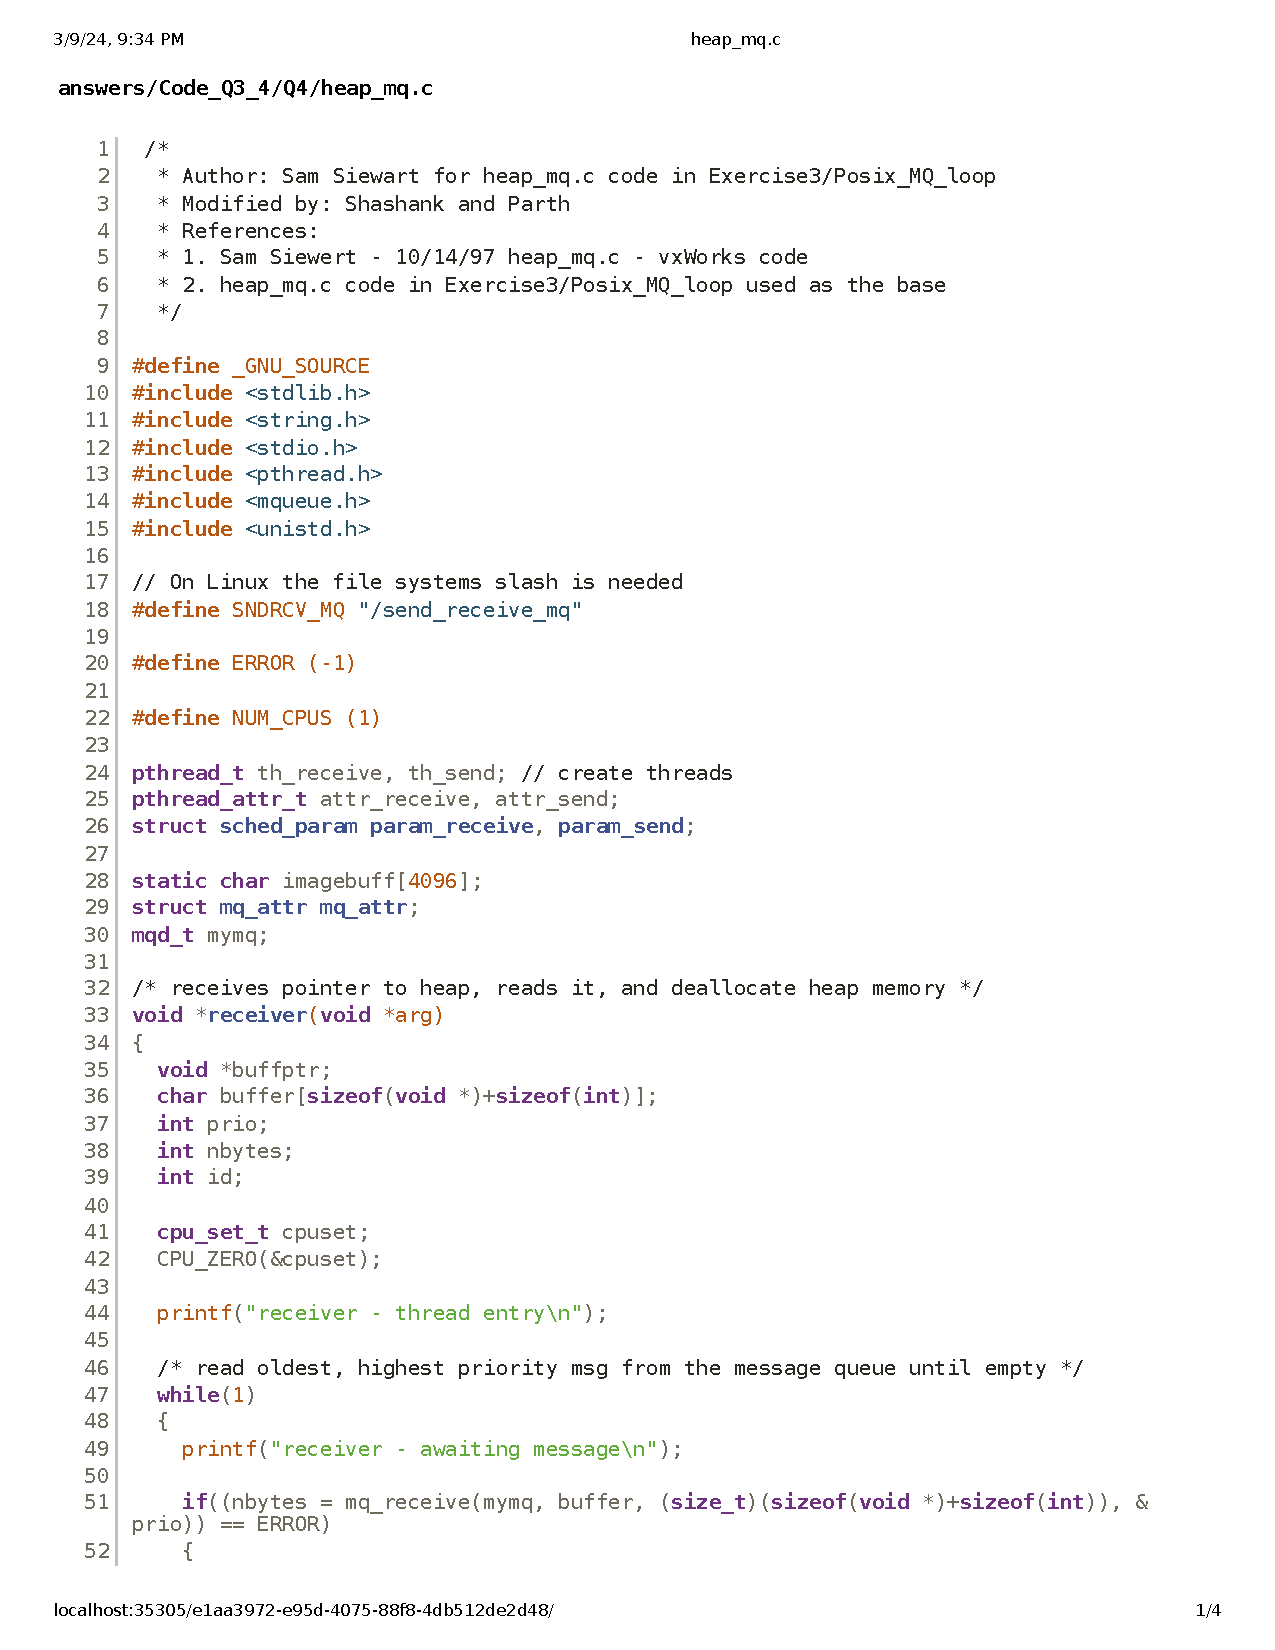
\includepdf[pages=-]{code/heap_mq.c.pdf}
	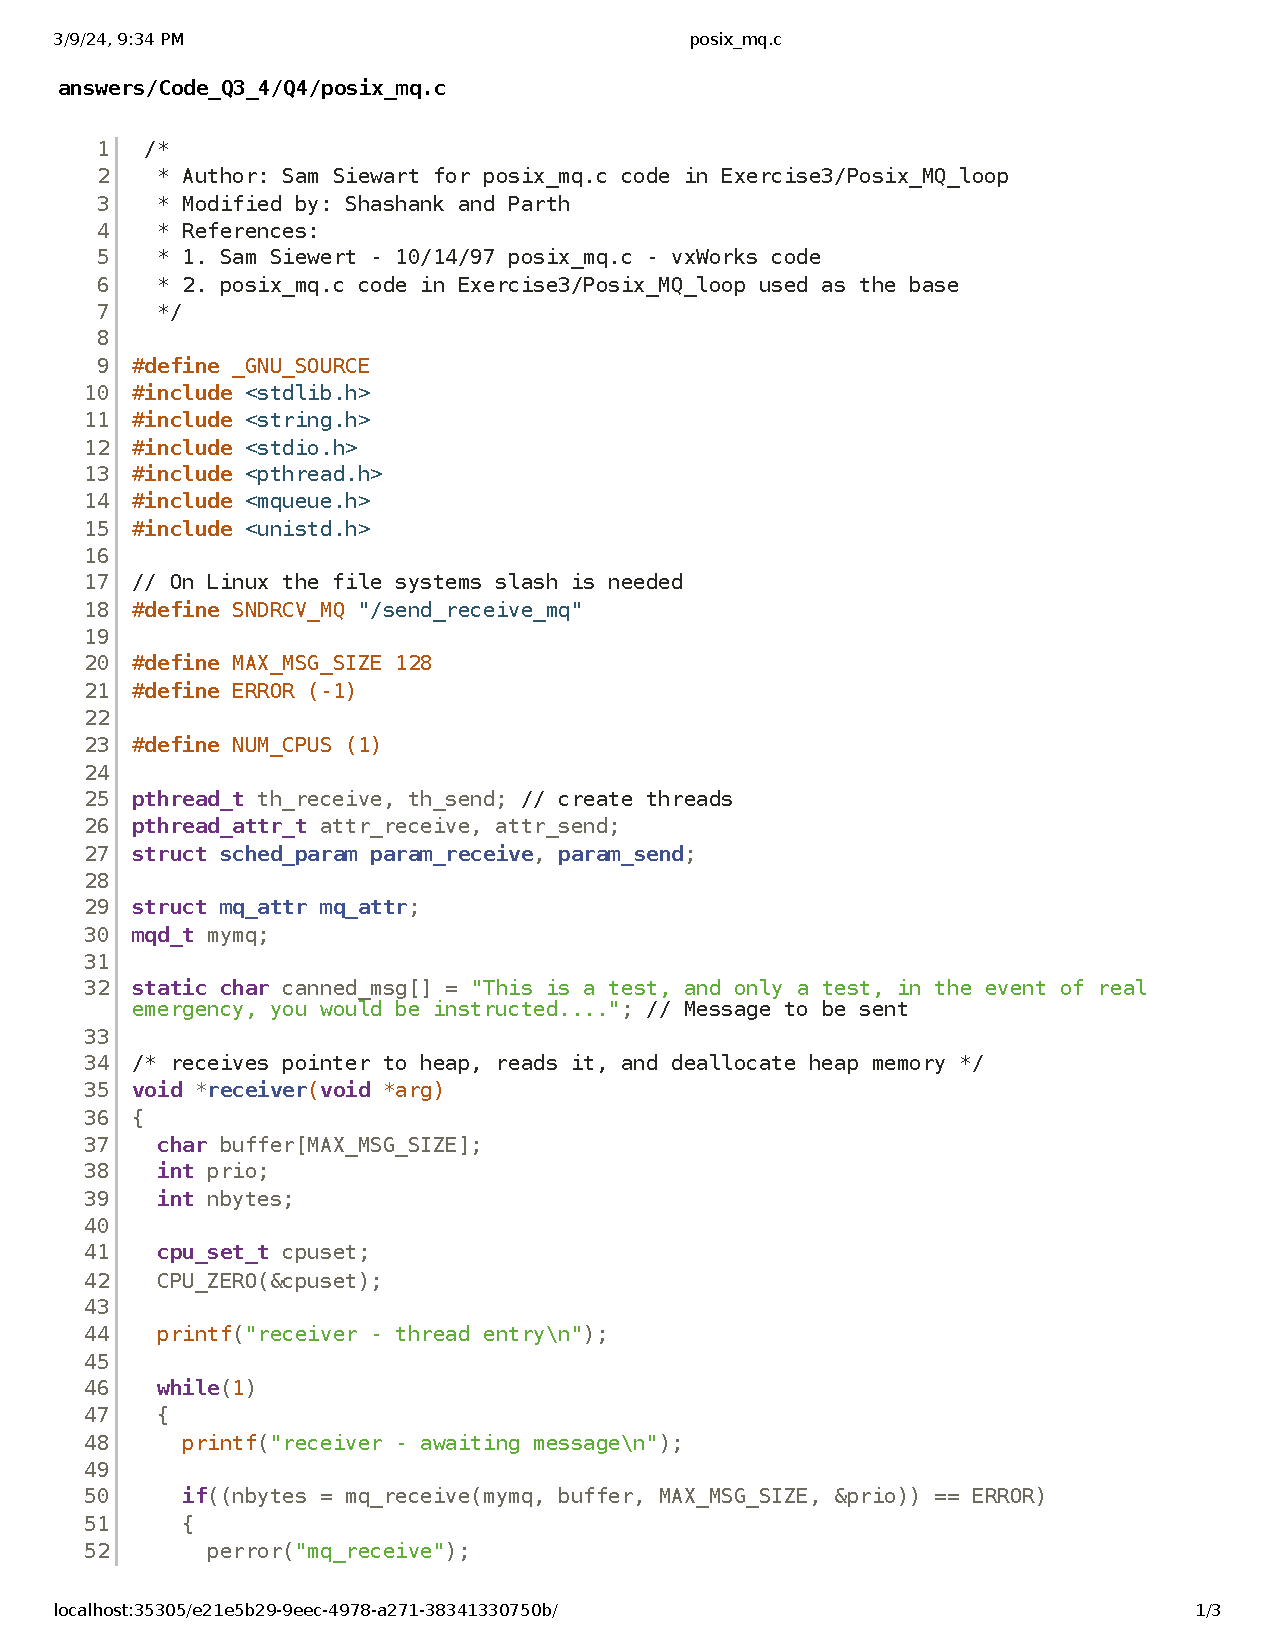
\includepdf[pages=-]{code/posix_mq.c.pdf}
	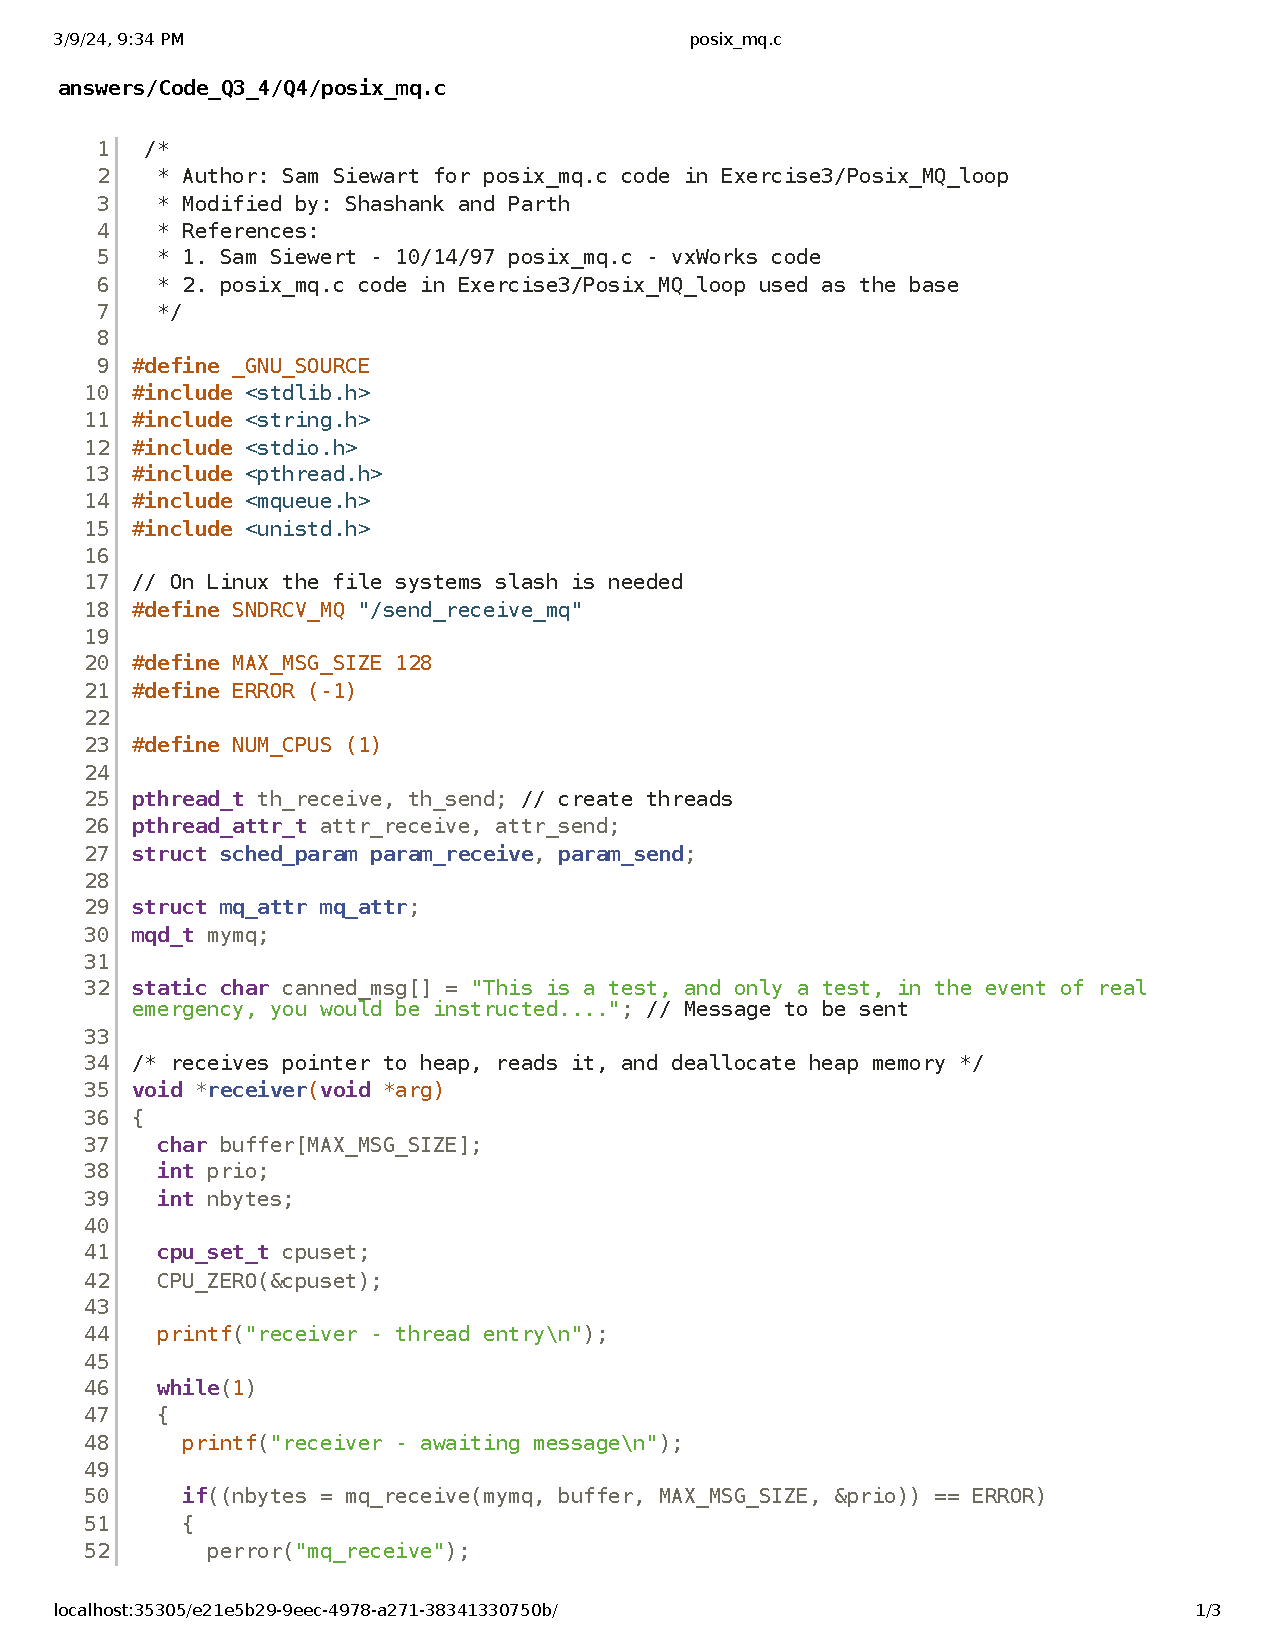
\includepdf[pages=-]{code/posix_mq.c.pdf}
	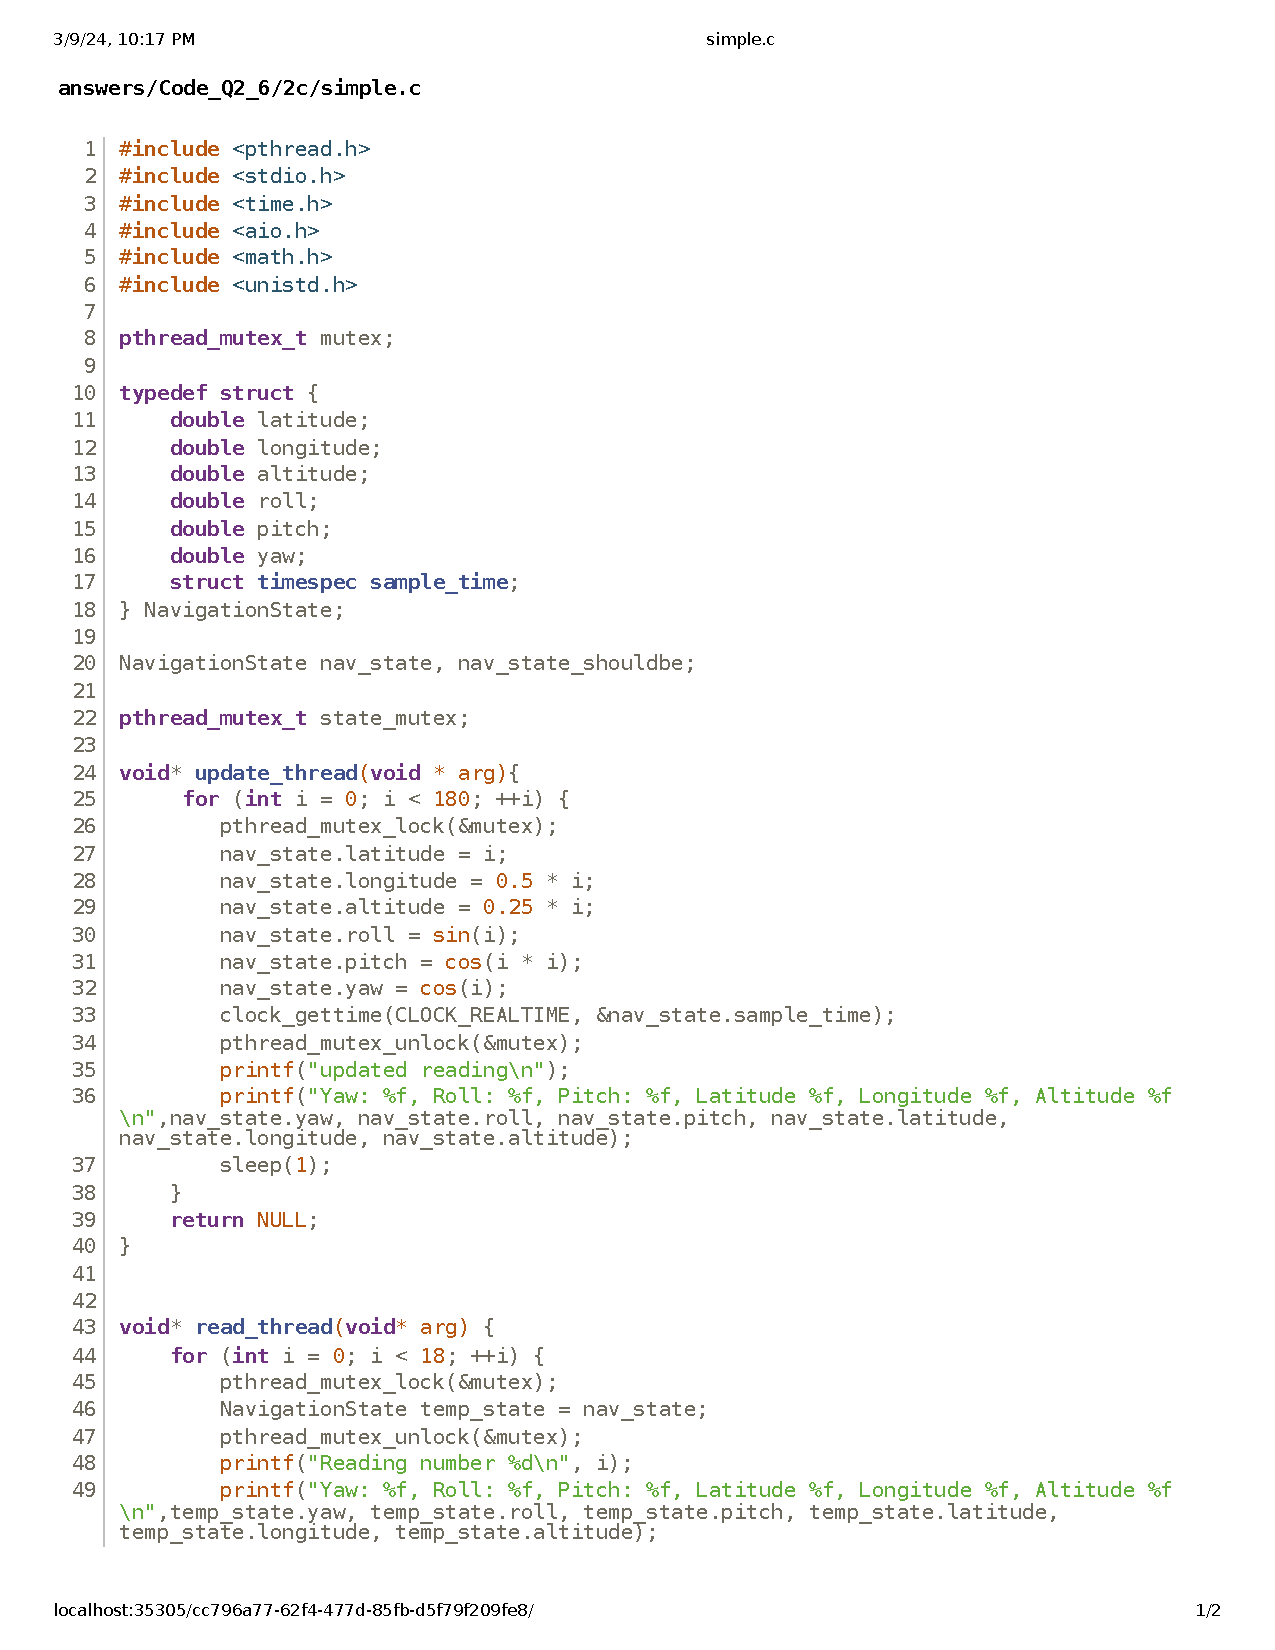
\includepdf[pages=-]{code/simple.c.pdf}
	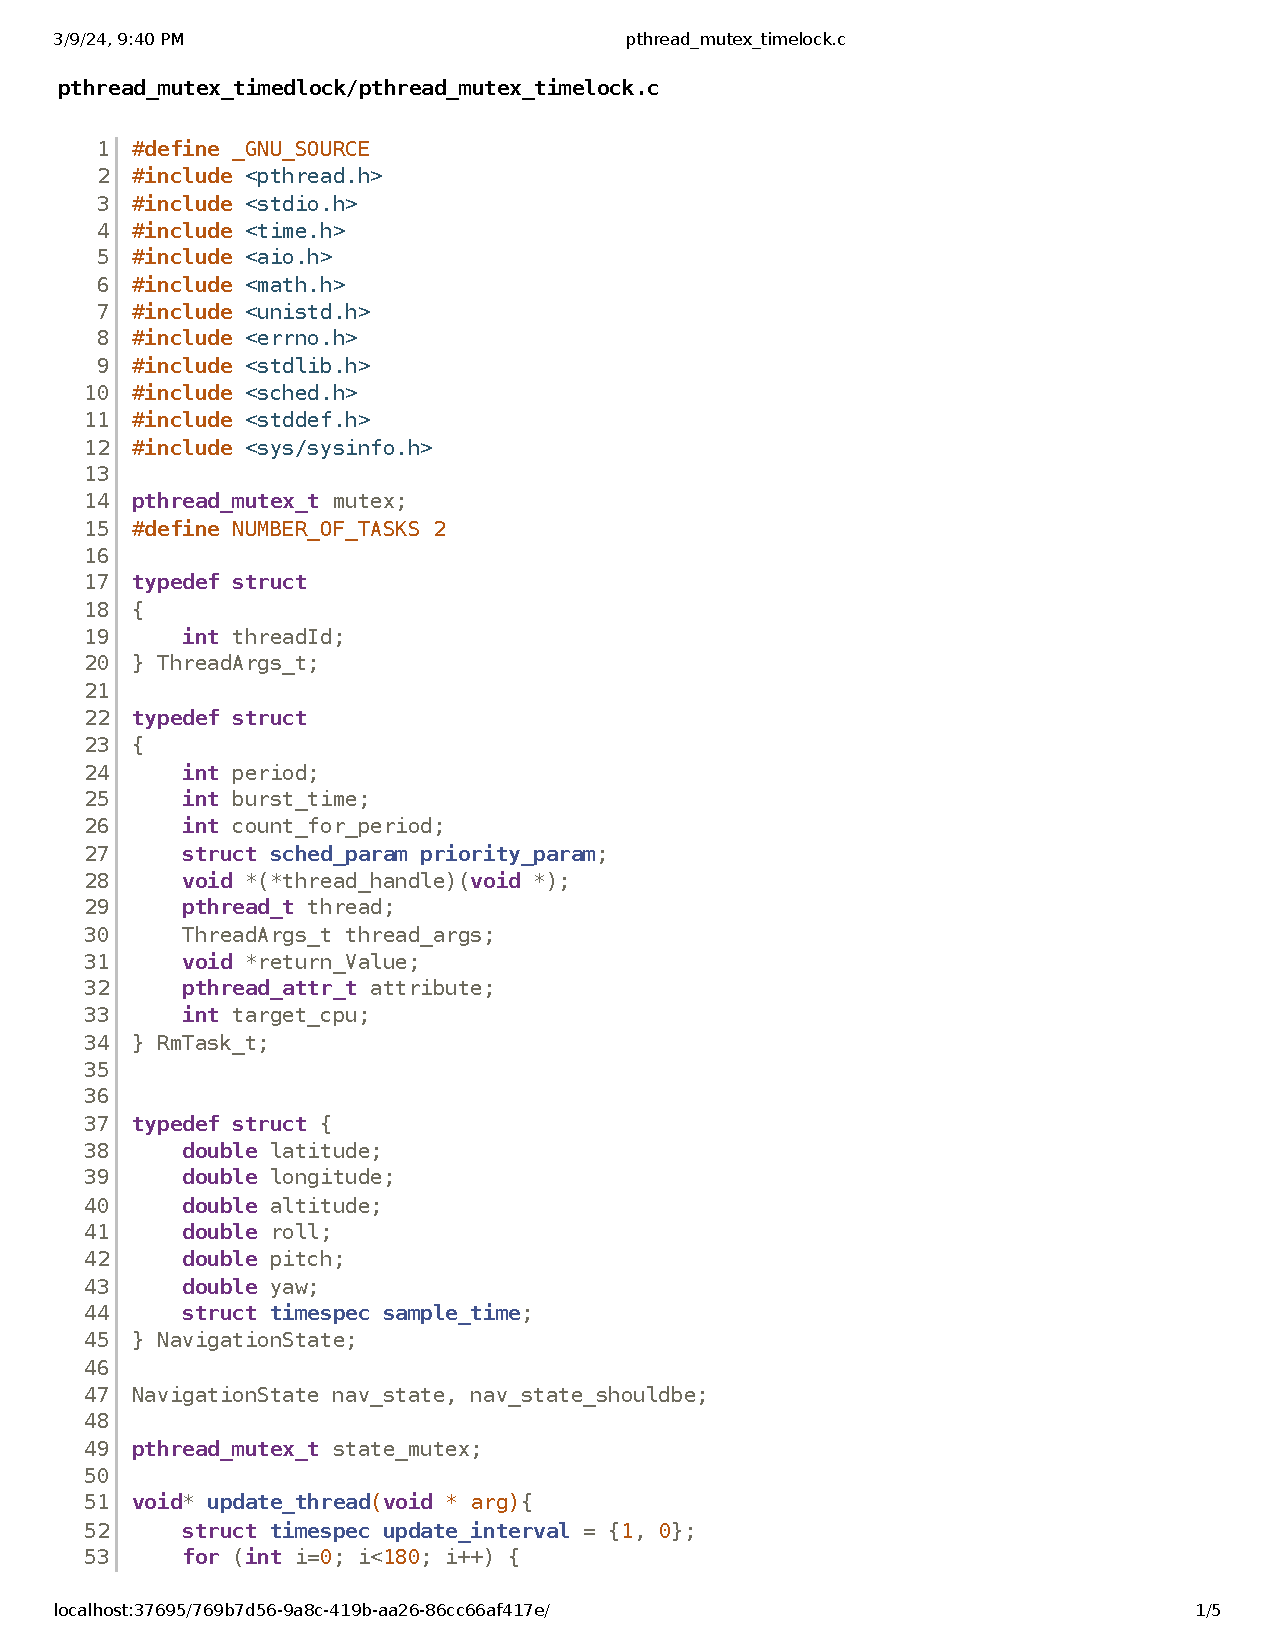
\includepdf[pages=-]{code/pthread_mutex_timelock.c.pdf}
\end{appendices}


\vspace{1cm}
\hrule
\vspace{0.5cm}


%---------------------------------------------------------------------------
\end{document}
-
